%%%%%%%%%%%%%%%%%%%%%%%%%%%%%%%%%%%%%%%%%%%%%%%%%%%%%%%%%%%%
%%  This Beamer template was created by Cameron Bracken.
%%  Anyone can freely use or modify it for any purpose
%%  without attribution.
%%
%%  Last Modified: January 9, 2009
%%

\documentclass[xcolor=x11names,compress]{beamer}

%% General document %%%%%%%%%%%%%%%%%%%%%%%%%%%%%%%%%%
\usepackage{graphicx}
\usepackage{tikz}
\usepackage{graphicx}
\usepackage{amsmath}

\usetikzlibrary{decorations.fractals}
%%%%%%%%%%%%%%%%%%%%%%%%%%%%%%%%%%%%%%%%%%%%%%%%%%%%%%


%% Beamer Layout %%%%%%%%%%%%%%%%%%%%%%%%%%%%%%%%%%
\useoutertheme[subsection=false,shadow]{miniframes}
\useinnertheme{default}
\usefonttheme{serif}
\usepackage{palatino}

\setbeamerfont{title like}{shape=\scshape}
\setbeamerfont{frametitle}{shape=\scshape}

\setbeamercolor*{lower separation line head}{bg=DeepSkyBlue4} 
\setbeamercolor*{normal text}{fg=black,bg=white} 
\setbeamercolor*{alerted text}{fg=red} 
\setbeamercolor*{example text}{fg=black} 
\setbeamercolor*{structure}{fg=black} 

\setbeamercolor*{palette tertiary}{fg=black,bg=black!10} 
\setbeamercolor*{palette quaternary}{fg=black,bg=black!10} 

\renewcommand{\(}{\begin{columns}}
\renewcommand{\)}{\end{columns}}
\newcommand{\<}[1]{\begin{column}{#1}}
\renewcommand{\>}{\end{column}}
%%%%%%%%%%%%%%%%%%%%%%%%%%%%%%%%%%%%%%%%%%%%%%%%%%


\begin{document}


%%%%%%%%%%%%%%%%%%%%%%%%%%%%%%%%%%%%%%%%%%%%%%%%%%%%%%

\begin{frame}
\title{QSEP Research Update}
%\subtitle{SUBTITLE}
\author{
	Halley Brantley\\
	{\it Savvy Sherpa}\\
}
\date{
	\begin{tikzpicture}[decoration=Koch curve type 2] 
	\draw[DeepSkyBlue4] decorate{ decorate{ decorate{ (0,0) -- (3,0) }}}; 
	\end{tikzpicture}  
	\\
	\vspace{1cm}
	\today
}
\titlepage
\end{frame}

\section{\scshape Overview}

\begin{frame}{Research Questions}
Original
\begin{itemize}
	\item Can we identify a dataset containing the pediatric illness populations of interest and their immediate family members? 
	\item Can we quantify the outcomes of interest and their relationship to the hypothesized mediating factors? 
	\item Do we see any significant secondary effects of pediatric illness on family members, in comparison to a sensibly-defined control group? 
\end{itemize}
Updated 
\begin{itemize}
	\item Do we see a difference in adult family member spending before and after a child is diagnosed?
\end{itemize}
\end{frame}

\section{\scshape Data}

\begin{frame}
Number of children under 16 with each condition, enrolled for more than 3 months, and for whom we have at least one month of spend data before diagnosis. 
\begin{itemize}
	\item Total sick children under 16: 136,791
	\item Unique Families: 122,588 
	\item Asthma:  87,872
	\item Autism (ASD): 8,732
	\item Cancer: 27,466
	\item Cerebral Palsy: 1,440
	\item Type 1 Diabetes (T1D): 1,434
	\item Traumatic Event: 22,313
	\item Multiple Conditions: 11,756
\end{itemize}	
\end{frame}

\begin{frame}{Data Cleaning }
\begin{itemize}
	\item To identify parents/guardians in the household used the criteria:
		\begin{itemize}
			\item Same household as sick child
			\item Older than 15
			\item At least 15 years older than the sick child 
			\item No more than 60 years older than the sick child
			\item Within 15 years of the age of the oldest member of the household
		\end{itemize} 
	\item Use months within 9 months of child's diagnosis. 
	\item Only include adult family members with at least 2 months of claims before diagnosis and 2 months after, including month of diagnosis. 
\end{itemize}
\end{frame}


\section{\scshape Modeling}

\begin{frame}{Models}
\begin{itemize}
	\item Goal: model monthly spend per adult family member before and after diagnosis.
	\item Approach: Use a hierarchical model
	\begin{enumerate}
		\item Model the probability that monthly spend is non-zero using logistic regression on confounders and 
		indicator of after diagnosis. 
		\item Conditioned on the fact that spend is non-zero model the total spend using lognormal regression on confounders and indicator of after diagnosis. 
	\end{enumerate}	
	\item Models were fit separately by gender of adult.
	\item Predictions are calculated as the predicted probability of non-zero spend multiplied by the predicted spend given that spend is non-zero. 
	\item Determine confidence intervals for predictions by bootstrapping (re-sample members with replacement and re-calculate predictions)
\end{itemize}
\end{frame}

\begin{frame}{Confounders}
\begin{itemize}
	\item RAF categories: 0, 0.5, 1, 2.5, 5, 10, 200 
	\item Income categories: 0, 50, 100, 150, 260 (thousands)
	\item Plan Type: Gated HMO, Choice Plus, Select Plus, Choice, Other
	\item Indicator of only one adult on the plan that meets the above criteria 
	\item Number of children on plan: 1, 2-4, 5+
	\item Indicator of multiple sick children
	\item Age category of youngest child: Infant, Child, Teenager
	\item Months Enrolled
	\item Time (natural spline)
	\item Adult age (natural spline)
\end{itemize}  
\end{frame}

\section{\scshape Results}

\begin{frame}{Predicted difference in mean monthly spend before and after diagnosis (\$)}
Averaged across all confounders.
%latex.default(CIs, colheads = c("", "Gender", "LB", "Mean", "UB"),     title = "", file = "../tables/pred_CIs.tex", na.blank = FALSE)%
\begin{table}[!tbp]
\begin{center}
\begin{tabular}{lllrrr}
\hline\hline
\multicolumn{1}{l}{}&\multicolumn{1}{c}{}&\multicolumn{1}{c}{Gender}&\multicolumn{1}{c}{LB}&\multicolumn{1}{c}{Mean}&\multicolumn{1}{c}{UB}\tabularnewline
\hline
1&T1D&female&$-326.60$&$-148.02$&$-75.96$\tabularnewline
2&T1D&female&$-121.33$&$ -55.46$&$-28.14$\tabularnewline
3&T1D&female&$-118.95$&$ -54.04$&$-27.56$\tabularnewline
4&Trauma&female&$ -98.66$&$ -67.82$&$-51.36$\tabularnewline
5&T1D&female&$ -75.50$&$ -34.38$&$-17.45$\tabularnewline
6&Trauma&female&$ -64.05$&$ -44.00$&$-33.30$\tabularnewline
7&Trauma&female&$ -41.84$&$ -28.61$&$-21.58$\tabularnewline
8&Cancer&female&$ -33.51$&$ -19.00$&$-10.32$\tabularnewline
9&Trauma&female&$ -29.13$&$ -19.92$&$-15.03$\tabularnewline
10&T1D&female&$ -23.83$&$ -10.77$&$ -4.60$\tabularnewline
11&T1D&male&$ -22.71$&$  10.19$&$ 63.42$\tabularnewline
12&Cancer&female&$ -21.74$&$ -12.25$&$ -6.58$\tabularnewline
13&Trauma&female&$ -20.46$&$ -12.93$&$ -8.59$\tabularnewline
14&Trauma&female&$ -19.16$&$ -12.05$&$ -7.94$\tabularnewline
15&T1D&female&$ -18.93$&$  -8.67$&$ -3.75$\tabularnewline
16&Cancer&female&$ -13.25$&$  -7.33$&$ -3.79$\tabularnewline
17&T1D&male&$ -11.08$&$  -1.43$&$ 12.49$\tabularnewline
18&Cancer&female&$  -8.14$&$  -4.45$&$ -2.24$\tabularnewline
19&T1D&male&$  -4.44$&$   2.45$&$ 13.72$\tabularnewline
20&Cancer&female&$  -2.56$&$  -1.05$&$ -0.28$\tabularnewline
21&Cancer&female&$  -2.55$&$  -1.05$&$ -0.28$\tabularnewline
22&T1D&male&$  -1.01$&$   2.44$&$  7.48$\tabularnewline
23&Cerebral&male&$   0.85$&$   2.82$&$  7.61$\tabularnewline
24&Trauma&male&$   1.09$&$   1.71$&$  2.54$\tabularnewline
25&T1D&male&$   1.14$&$   2.16$&$  3.54$\tabularnewline
26&Trauma&male&$   1.20$&$   1.85$&$  2.71$\tabularnewline
27&Asthma&male&$   1.20$&$   2.09$&$  3.28$\tabularnewline
28&Asthma&male&$   1.22$&$   2.09$&$  3.24$\tabularnewline
29&Cerebral&male&$   1.30$&$   4.00$&$ 10.53$\tabularnewline
30&Cancer&male&$   1.33$&$   2.26$&$  3.68$\tabularnewline
31&Cancer&male&$   1.34$&$   2.29$&$  3.73$\tabularnewline
32&T1D&male&$   1.40$&$   2.49$&$  4.07$\tabularnewline
33&ASD&male&$   1.94$&$   3.41$&$  5.32$\tabularnewline
34&ASD&male&$   2.13$&$   3.75$&$  5.86$\tabularnewline
35&ASD&female&$   2.58$&$   3.92$&$  5.69$\tabularnewline
36&ASD&female&$   2.74$&$   4.18$&$  6.10$\tabularnewline
37&Asthma&female&$   3.28$&$   5.01$&$  8.05$\tabularnewline
38&Asthma&female&$   3.37$&$   5.15$&$  8.28$\tabularnewline
39&ASD&female&$   3.38$&$   5.05$&$  8.06$\tabularnewline
40&Asthma&male&$   3.53$&$   4.52$&$  6.42$\tabularnewline
41&Cancer&male&$   4.07$&$   5.01$&$  6.72$\tabularnewline
42&Cerebral&male&$   4.31$&$  12.00$&$ 29.79$\tabularnewline
43&Trauma&male&$   4.38$&$   5.34$&$  6.63$\tabularnewline
44&ASD&female&$   4.88$&$   7.33$&$ 11.78$\tabularnewline
45&Asthma&male&$   5.18$&$   6.70$&$  9.95$\tabularnewline
46&Cancer&male&$   6.07$&$   7.46$&$ 10.12$\tabularnewline
47&Asthma&female&$   6.10$&$   8.63$&$ 13.46$\tabularnewline
48&Trauma&male&$   6.92$&$   8.38$&$ 10.54$\tabularnewline
49&Cerebral&female&$   7.02$&$  11.52$&$ 18.40$\tabularnewline
50&ASD&male&$   7.13$&$   9.33$&$ 13.46$\tabularnewline
51&Asthma&male&$   8.02$&$  10.38$&$ 15.39$\tabularnewline
52&ASD&female&$   8.02$&$  12.11$&$ 19.51$\tabularnewline
53&Cerebral&female&$   8.04$&$  12.90$&$ 20.22$\tabularnewline
54&Cancer&male&$   8.68$&$  10.80$&$ 15.08$\tabularnewline
55&Cerebral&male&$   8.80$&$  24.42$&$ 60.67$\tabularnewline
56&Asthma&female&$   9.32$&$  13.12$&$ 20.35$\tabularnewline
57&Trauma&male&$   9.99$&$  12.07$&$ 15.21$\tabularnewline
58&ASD&male&$  11.77$&$  15.62$&$ 23.42$\tabularnewline
59&ASD&female&$  13.85$&$  20.87$&$ 33.60$\tabularnewline
60&Asthma&male&$  14.40$&$  18.73$&$ 28.28$\tabularnewline
61&Cerebral&male&$  14.44$&$  39.38$&$ 98.05$\tabularnewline
62&Asthma&female&$  15.50$&$  21.80$&$ 33.77$\tabularnewline
63&Cerebral&female&$  15.74$&$  24.11$&$ 36.07$\tabularnewline
64&Cancer&male&$  16.01$&$  19.99$&$ 28.16$\tabularnewline
65&Cerebral&male&$  16.48$&$  46.16$&$114.42$\tabularnewline
66&Trauma&male&$  16.76$&$  20.22$&$ 25.78$\tabularnewline
67&ASD&male&$  18.48$&$  24.33$&$ 35.59$\tabularnewline
68&Asthma&female&$  21.82$&$  30.69$&$ 47.56$\tabularnewline
69&Cerebral&female&$  28.44$&$  43.54$&$ 65.10$\tabularnewline
70&ASD&male&$  34.39$&$  44.88$&$ 64.86$\tabularnewline
71&Cerebral&female&$  44.33$&$  67.82$&$101.36$\tabularnewline
72&Cerebral&female&$  51.08$&$  77.94$&$116.10$\tabularnewline
\hline
\end{tabular}\end{center}
\end{table}

\end{frame}

\begin{frame}{Factor Increase in odds of depression }
95\% confidence intervals
%latex.default(combined_depress, title = "", rowname = NULL, file = "../tables/odds_depression.tex",     na.blank = FALSE)%
\begin{table}[!tbp]
\begin{center}
\begin{tabular}{llrrr}
\hline\hline
\multicolumn{1}{c}{Condition}&\multicolumn{1}{c}{Gender}&\multicolumn{1}{c}{LB}&\multicolumn{1}{c}{estimate}&\multicolumn{1}{c}{UB}\tabularnewline
\hline
ASD&male&$0.93$&$1.00$&$1.06$\tabularnewline
ASD&female&$0.99$&$1.04$&$1.09$\tabularnewline
Asthma&male&$1.01$&$1.04$&$1.07$\tabularnewline
Asthma&female&$1.03$&$1.04$&$1.06$\tabularnewline
Cerebral&male&$0.76$&$0.93$&$1.13$\tabularnewline
Cerebral&female&$1.14$&$1.31$&$1.50$\tabularnewline
CA&male&$0.99$&$1.03$&$1.07$\tabularnewline
CA&female&$1.05$&$1.08$&$1.11$\tabularnewline
Trauma&male&$0.91$&$0.95$&$0.98$\tabularnewline
Trauma&female&$1.05$&$1.08$&$1.11$\tabularnewline
T1D&male&$0.77$&$0.99$&$1.28$\tabularnewline
T1D&female&$0.93$&$1.10$&$1.29$\tabularnewline
\hline
\end{tabular}\end{center}
\end{table}

\end{frame}

\begin{frame}{ASD effect on men's spending}
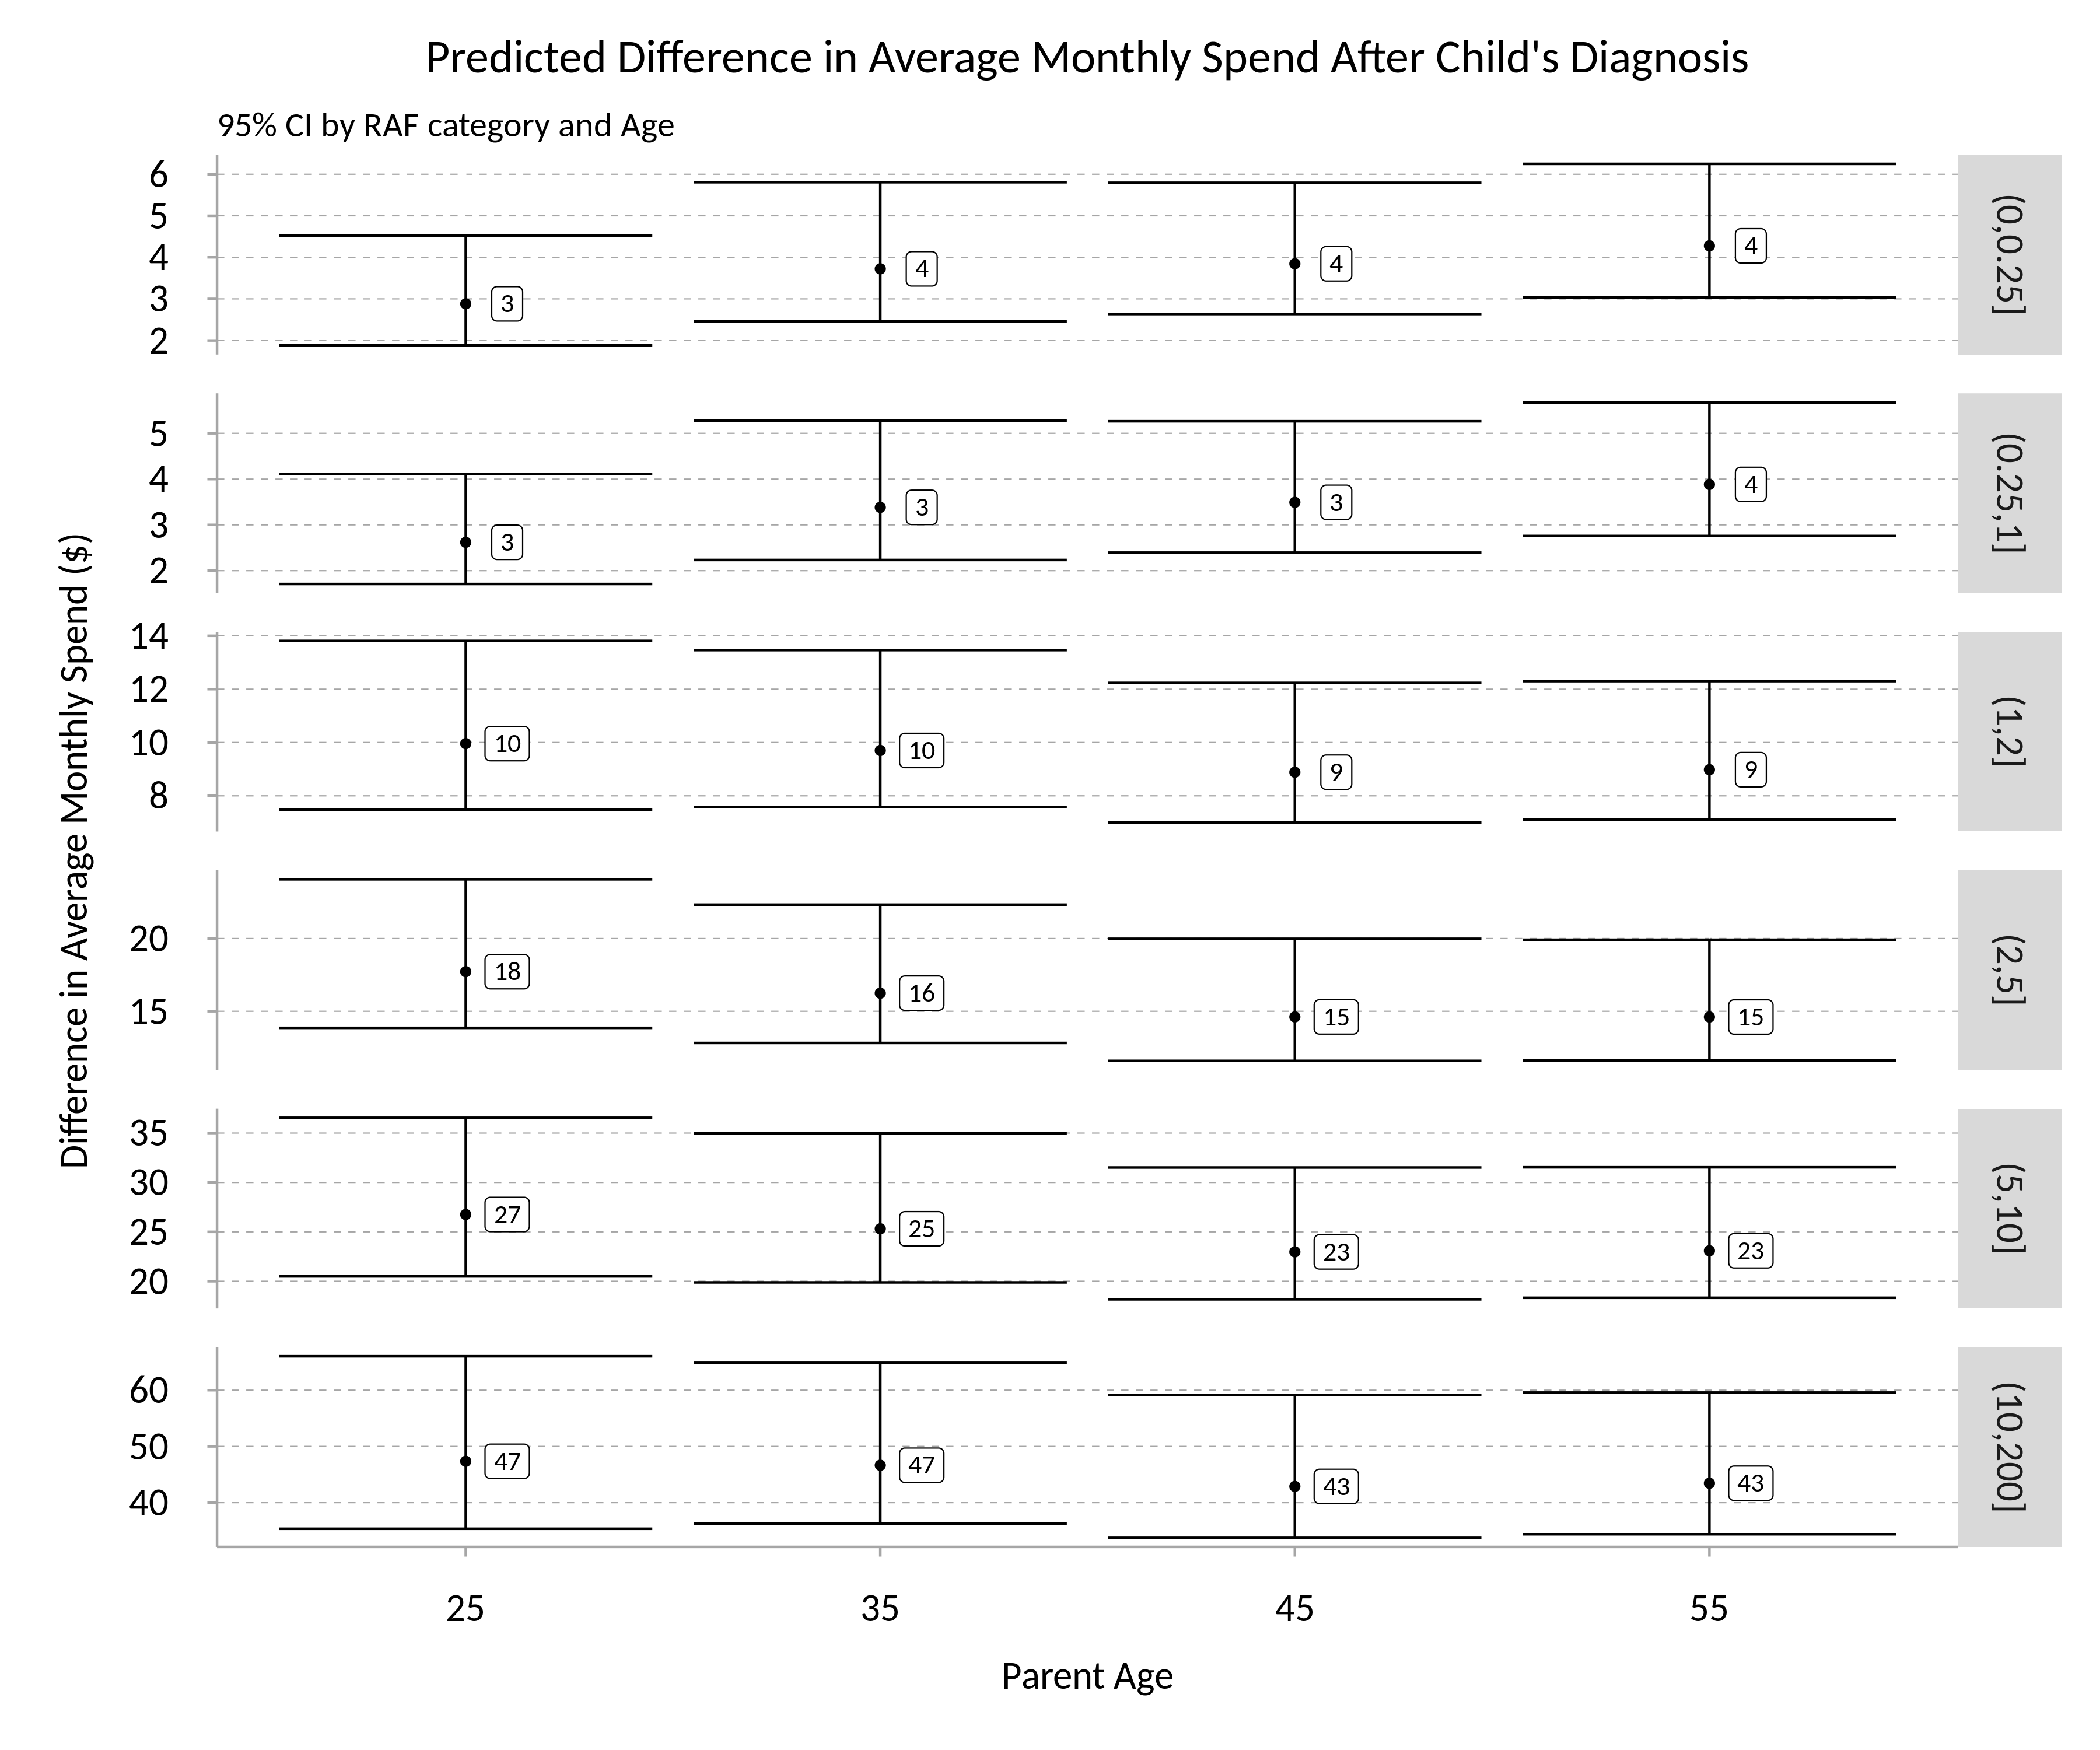
\includegraphics[width=.75\linewidth]{../figures/predicted_spend_male_ASD.png}
\end{frame}

\begin{frame}{ASD effect on women's spending}
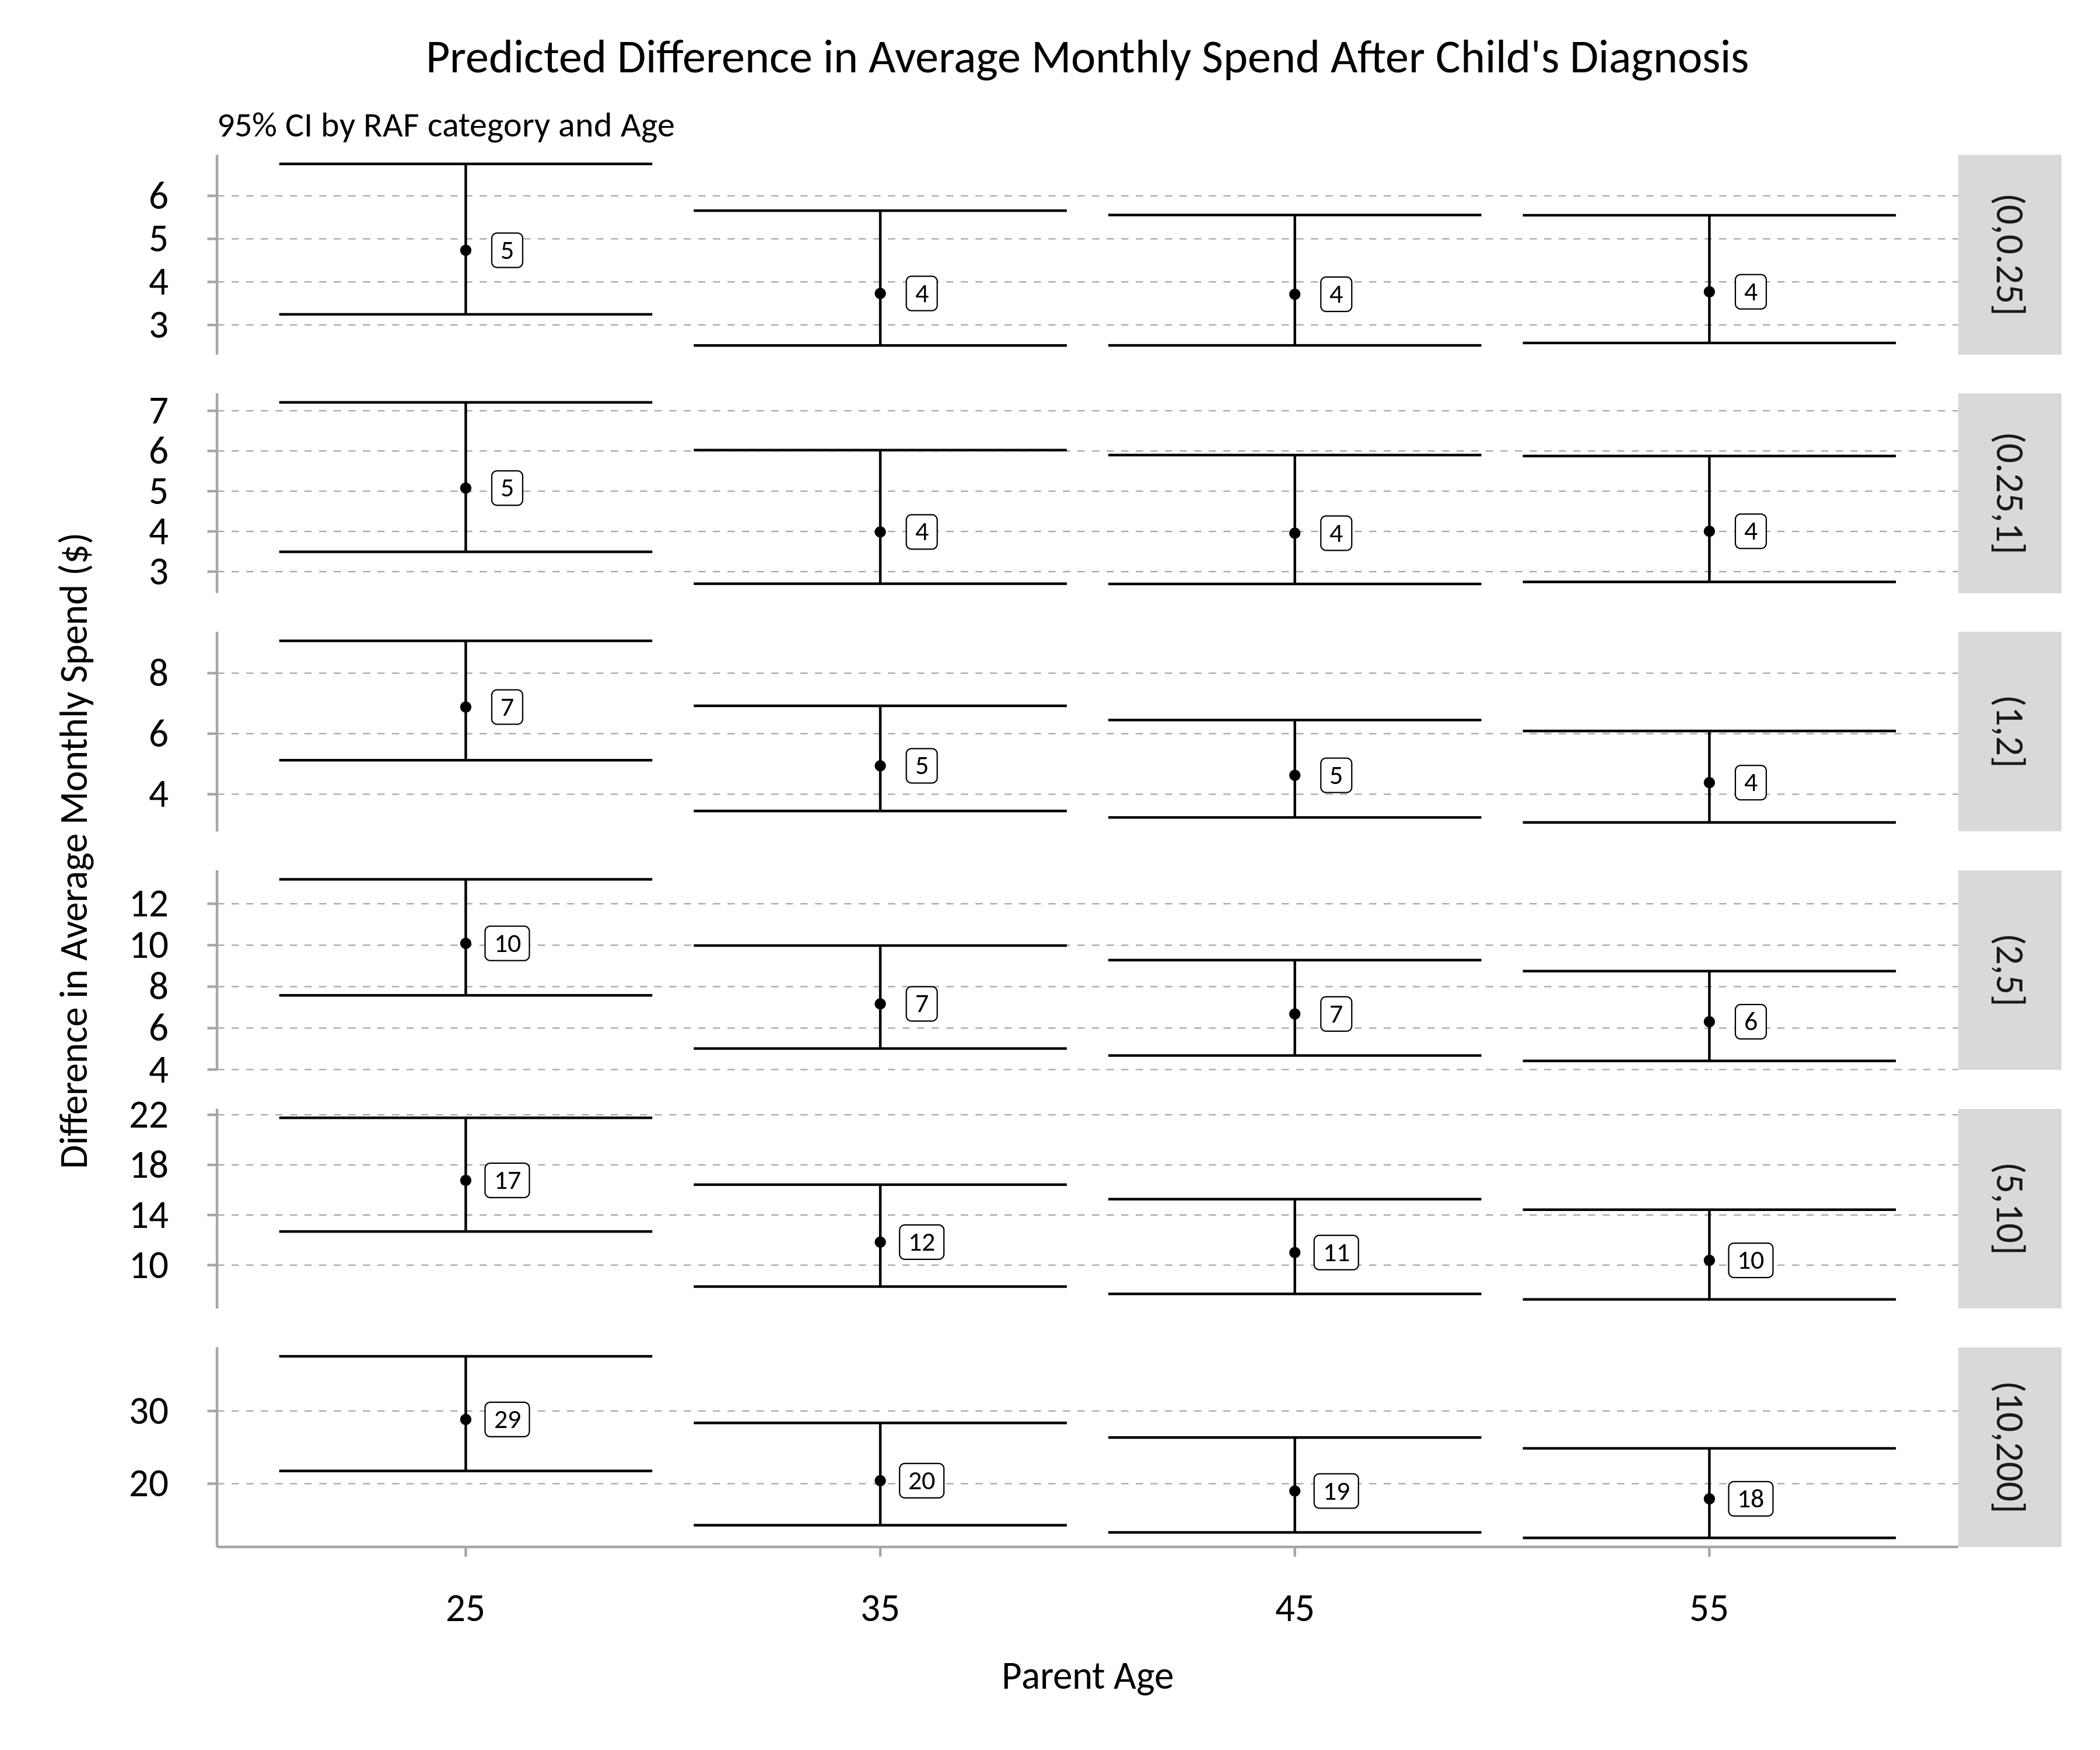
\includegraphics[width=.75\linewidth]{../figures/predicted_spend_female_ASD.png}
\end{frame}

\begin{frame}{Cerebral Palsy effect on men's spending}
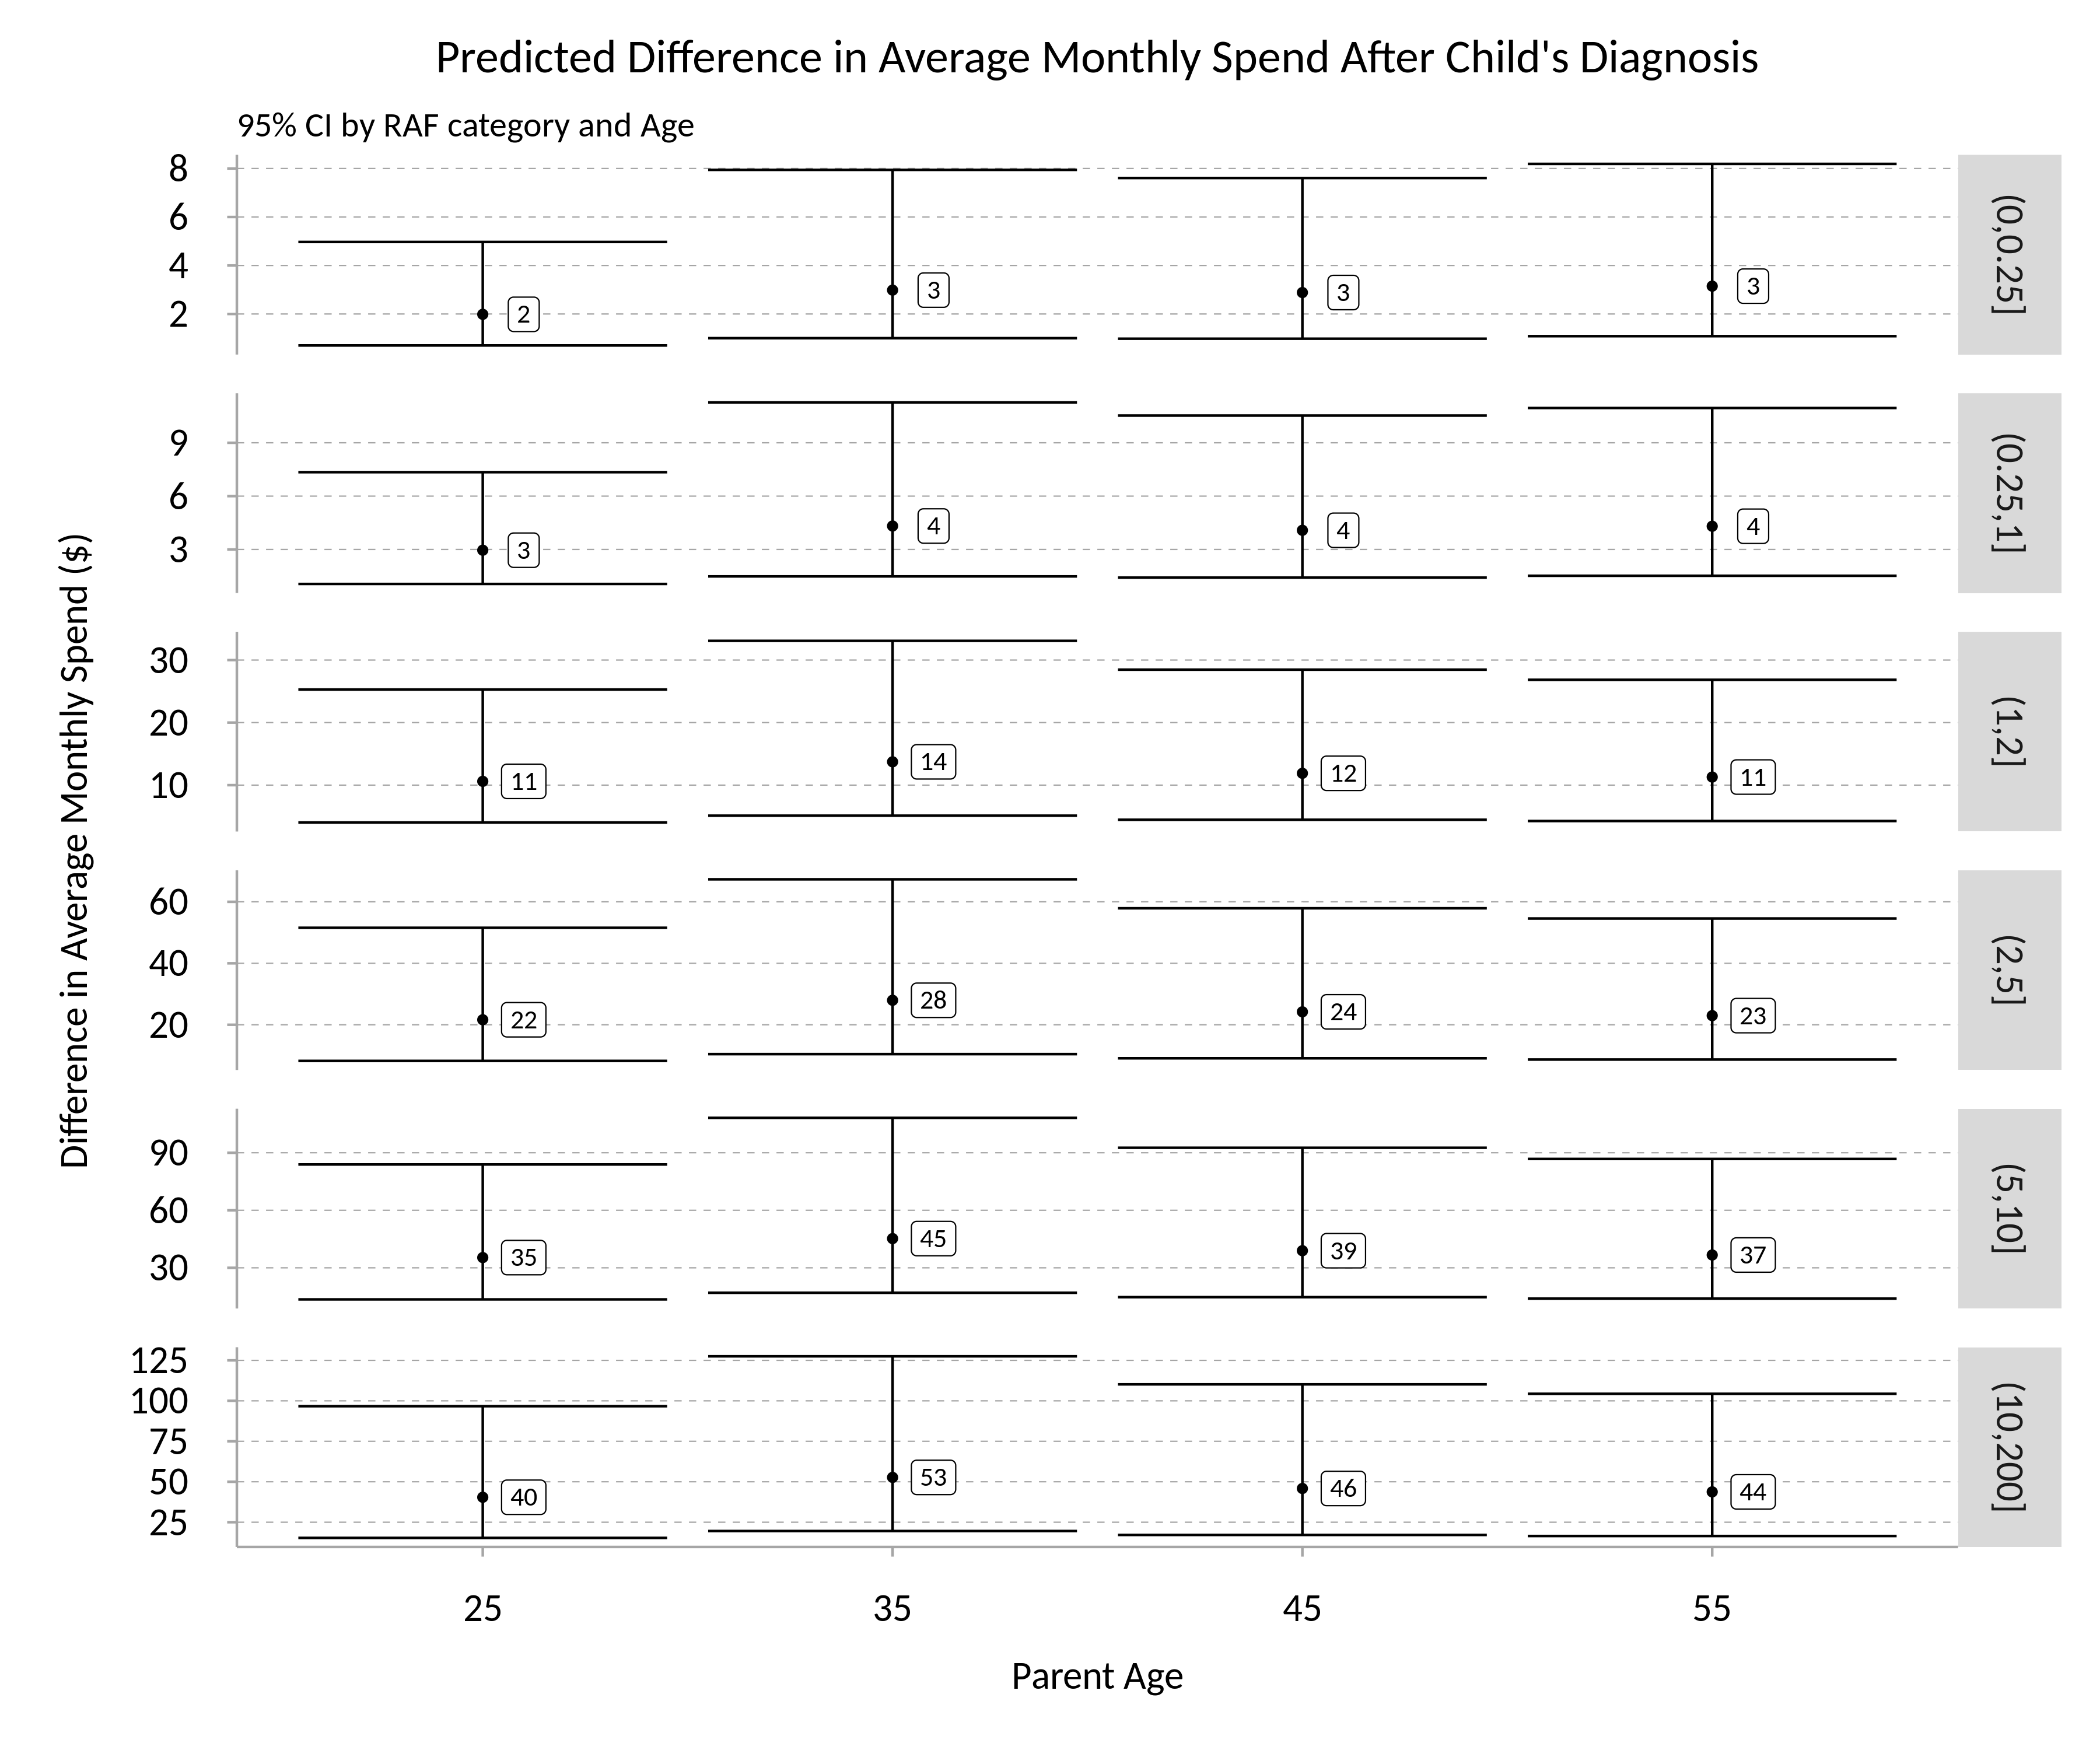
\includegraphics[width=.75\linewidth]{../figures/predicted_spend_male_Cerebral.png}
\end{frame}

\begin{frame}{Cerebral Palsy effect on women's spending}
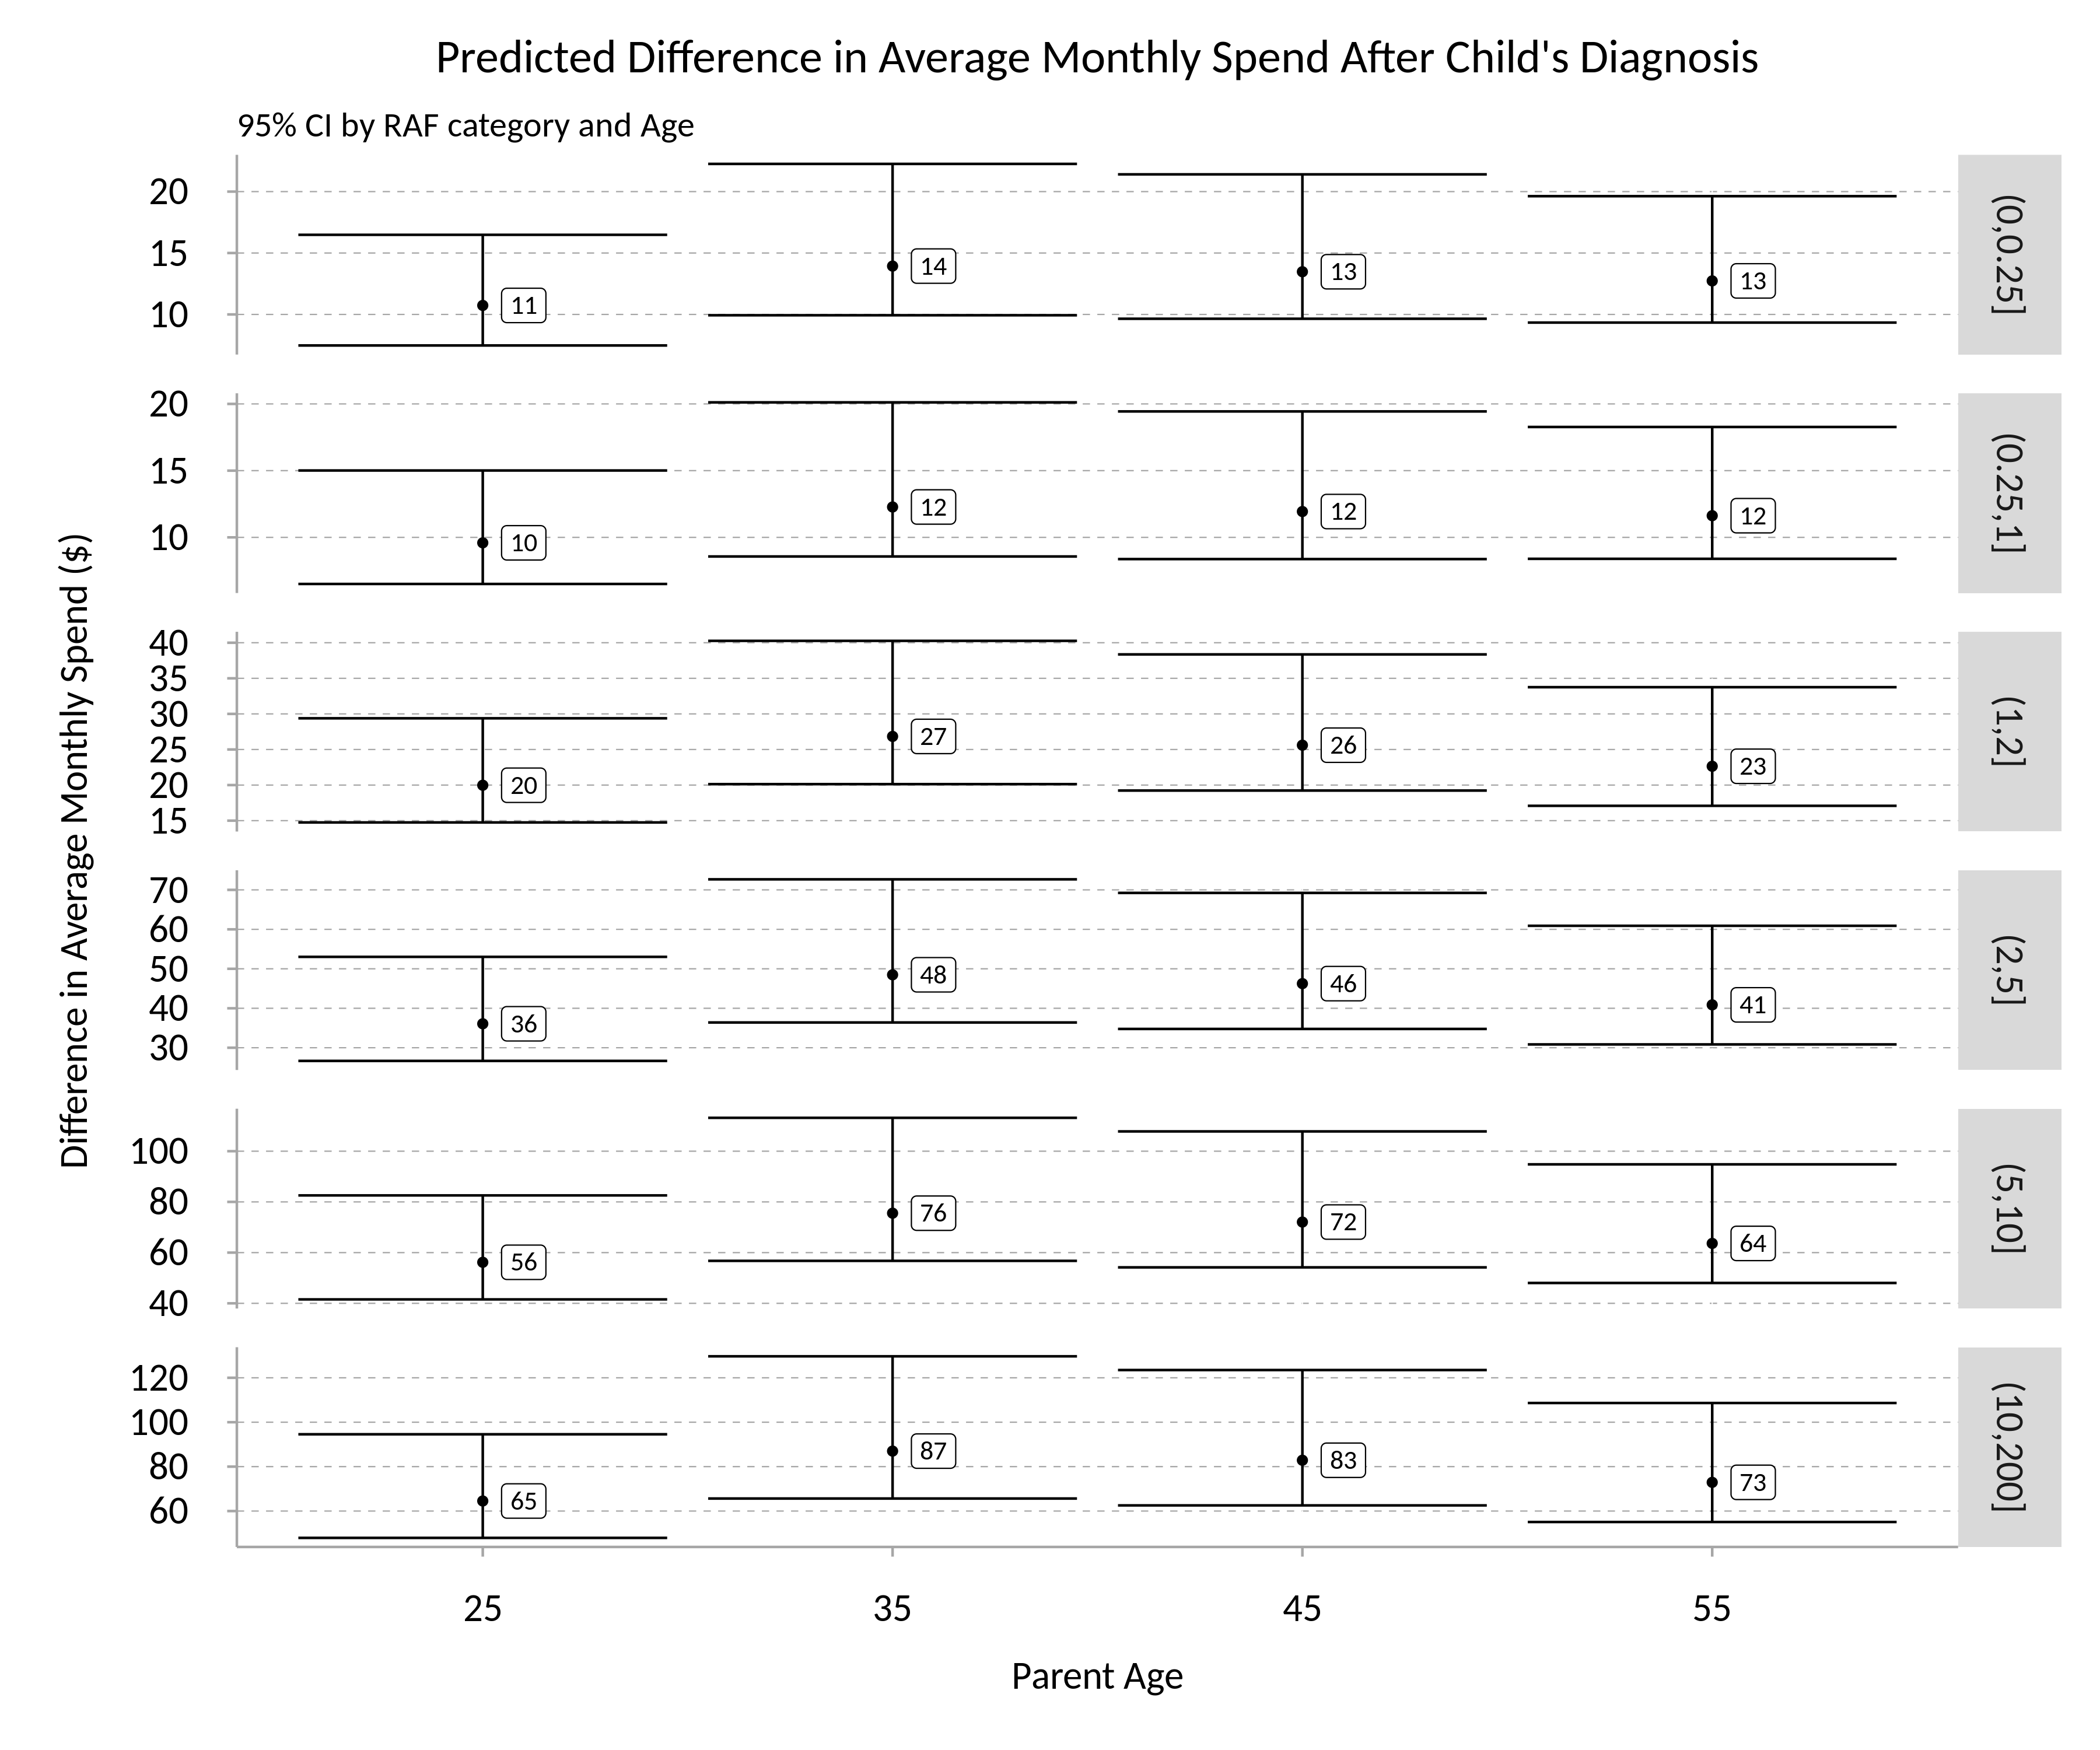
\includegraphics[width=.75\linewidth]{../figures/predicted_spend_female_Cerebral.png}
\end{frame}

\begin{frame}{Cancer effect on men's spending}
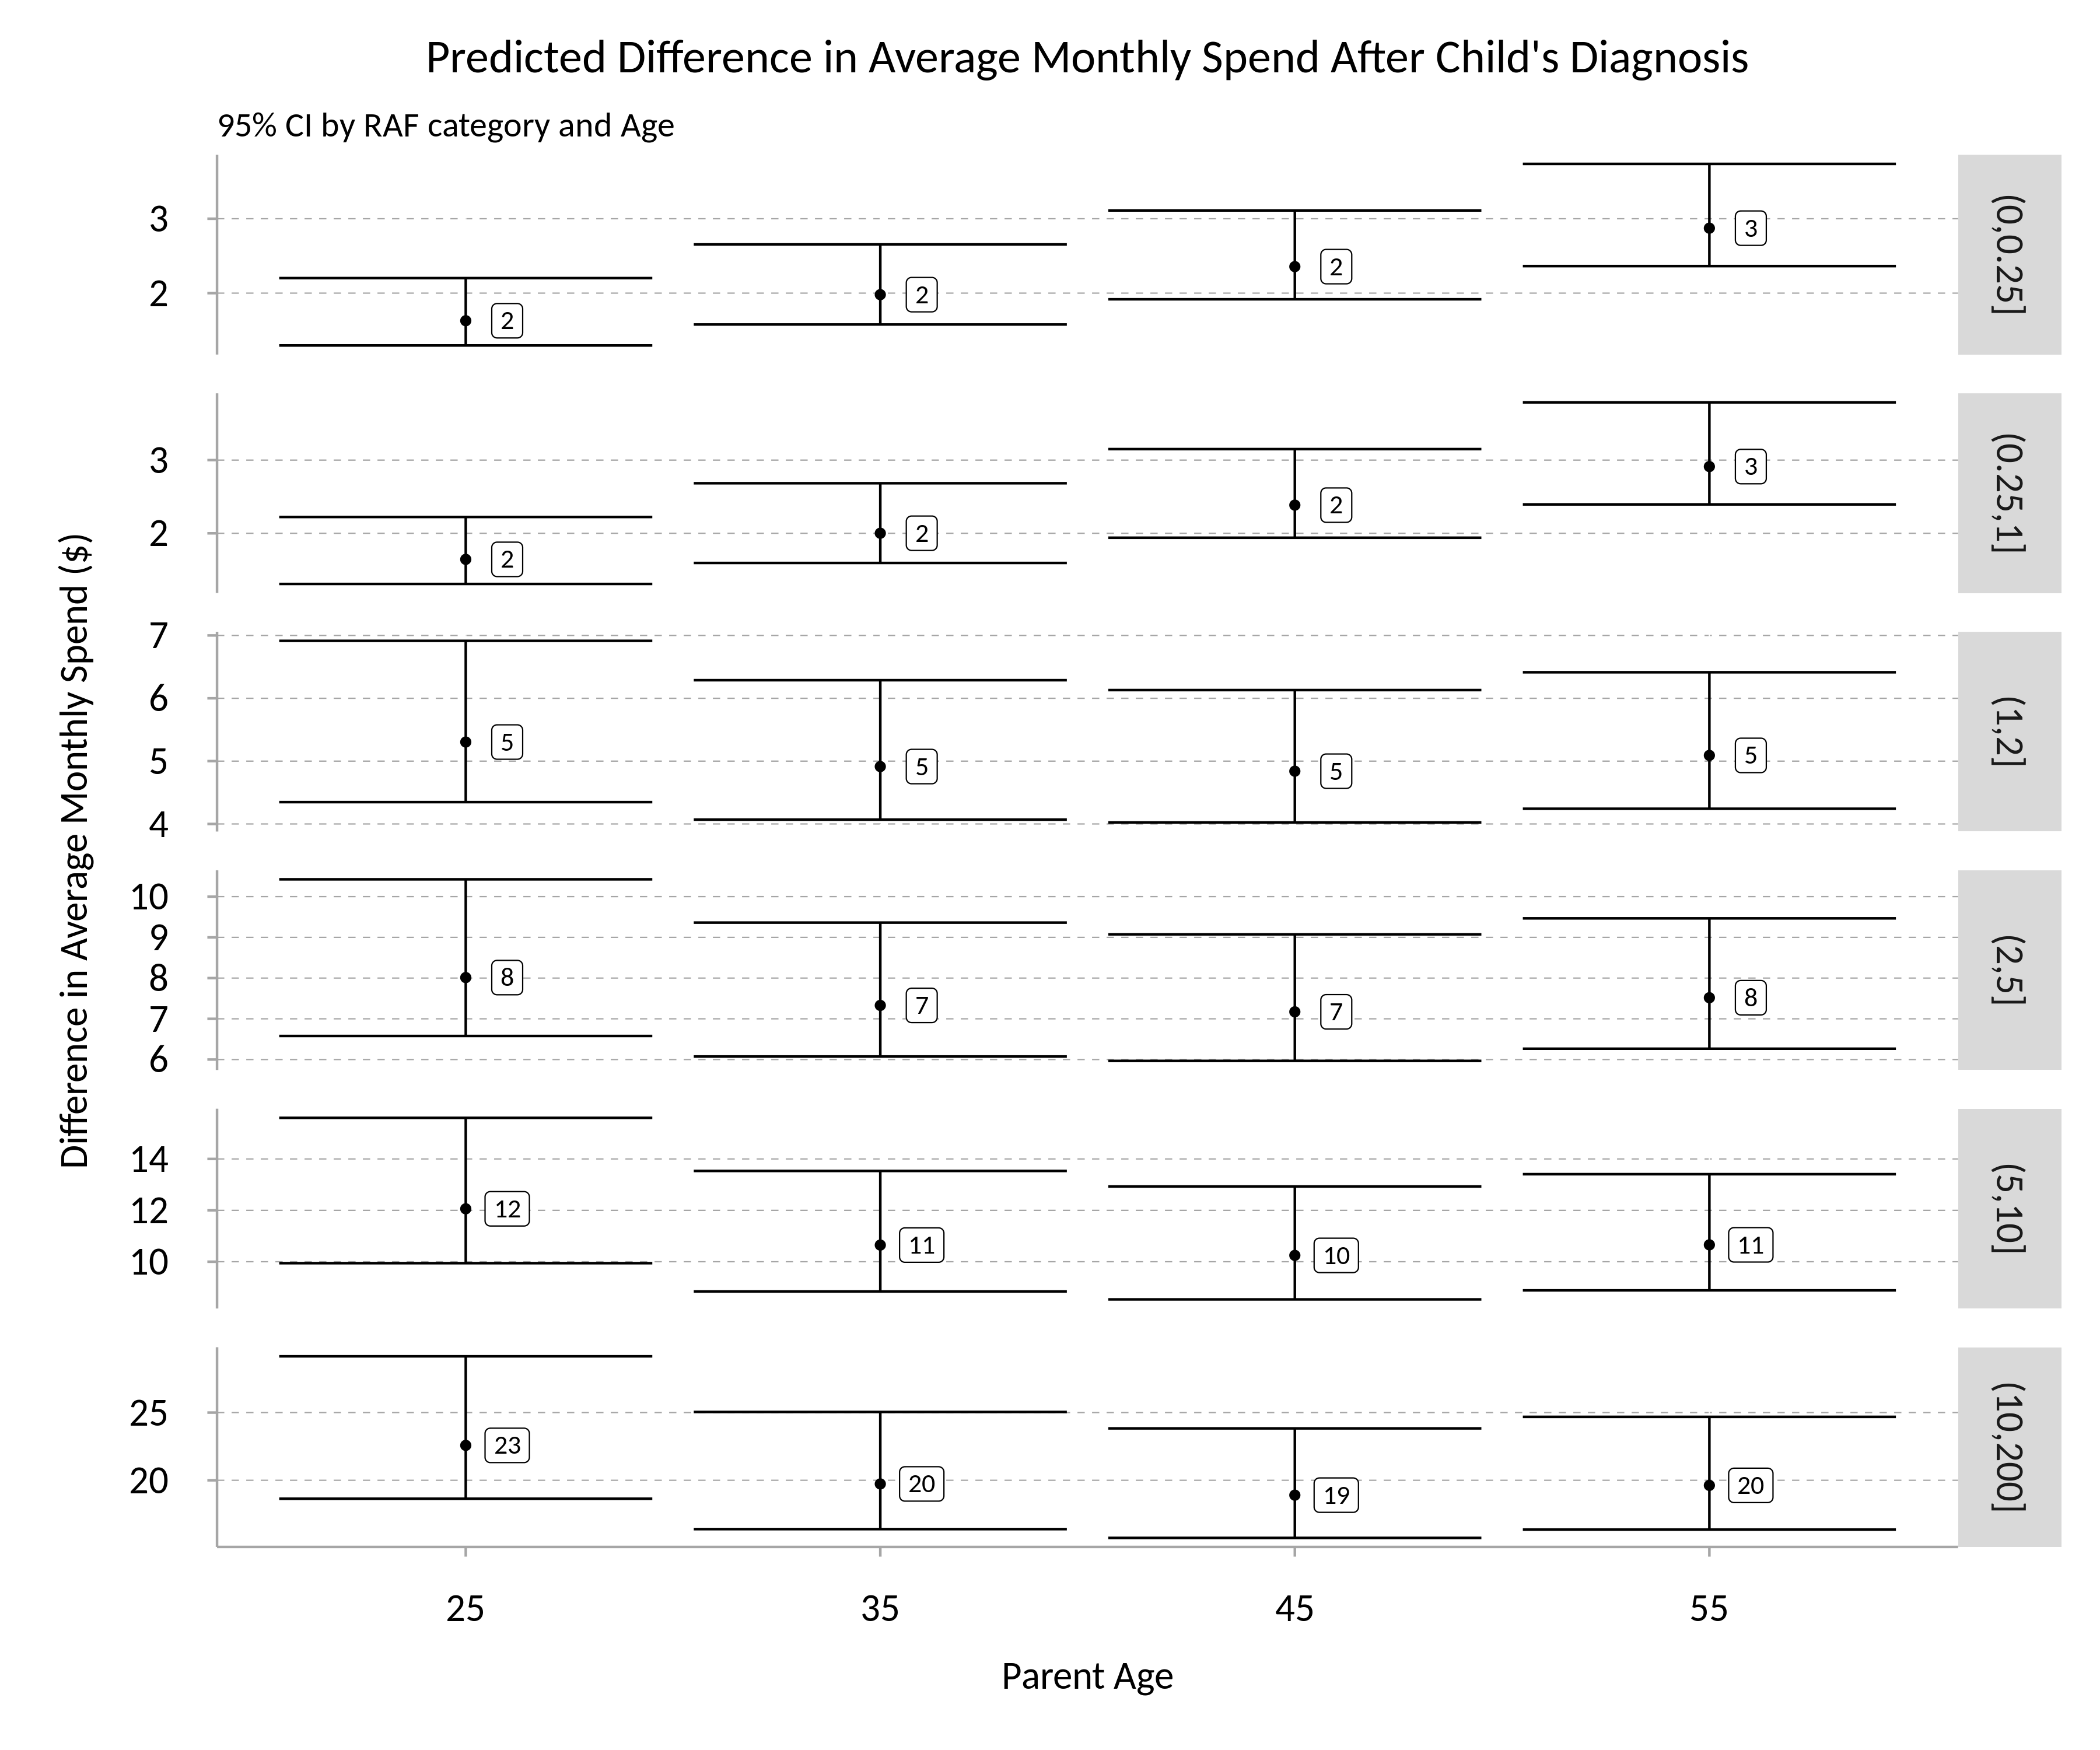
\includegraphics[width=.75\linewidth]{../figures/predicted_spend_male_CA.png}
\end{frame}

\begin{frame}{Cancer effect on women's spending}
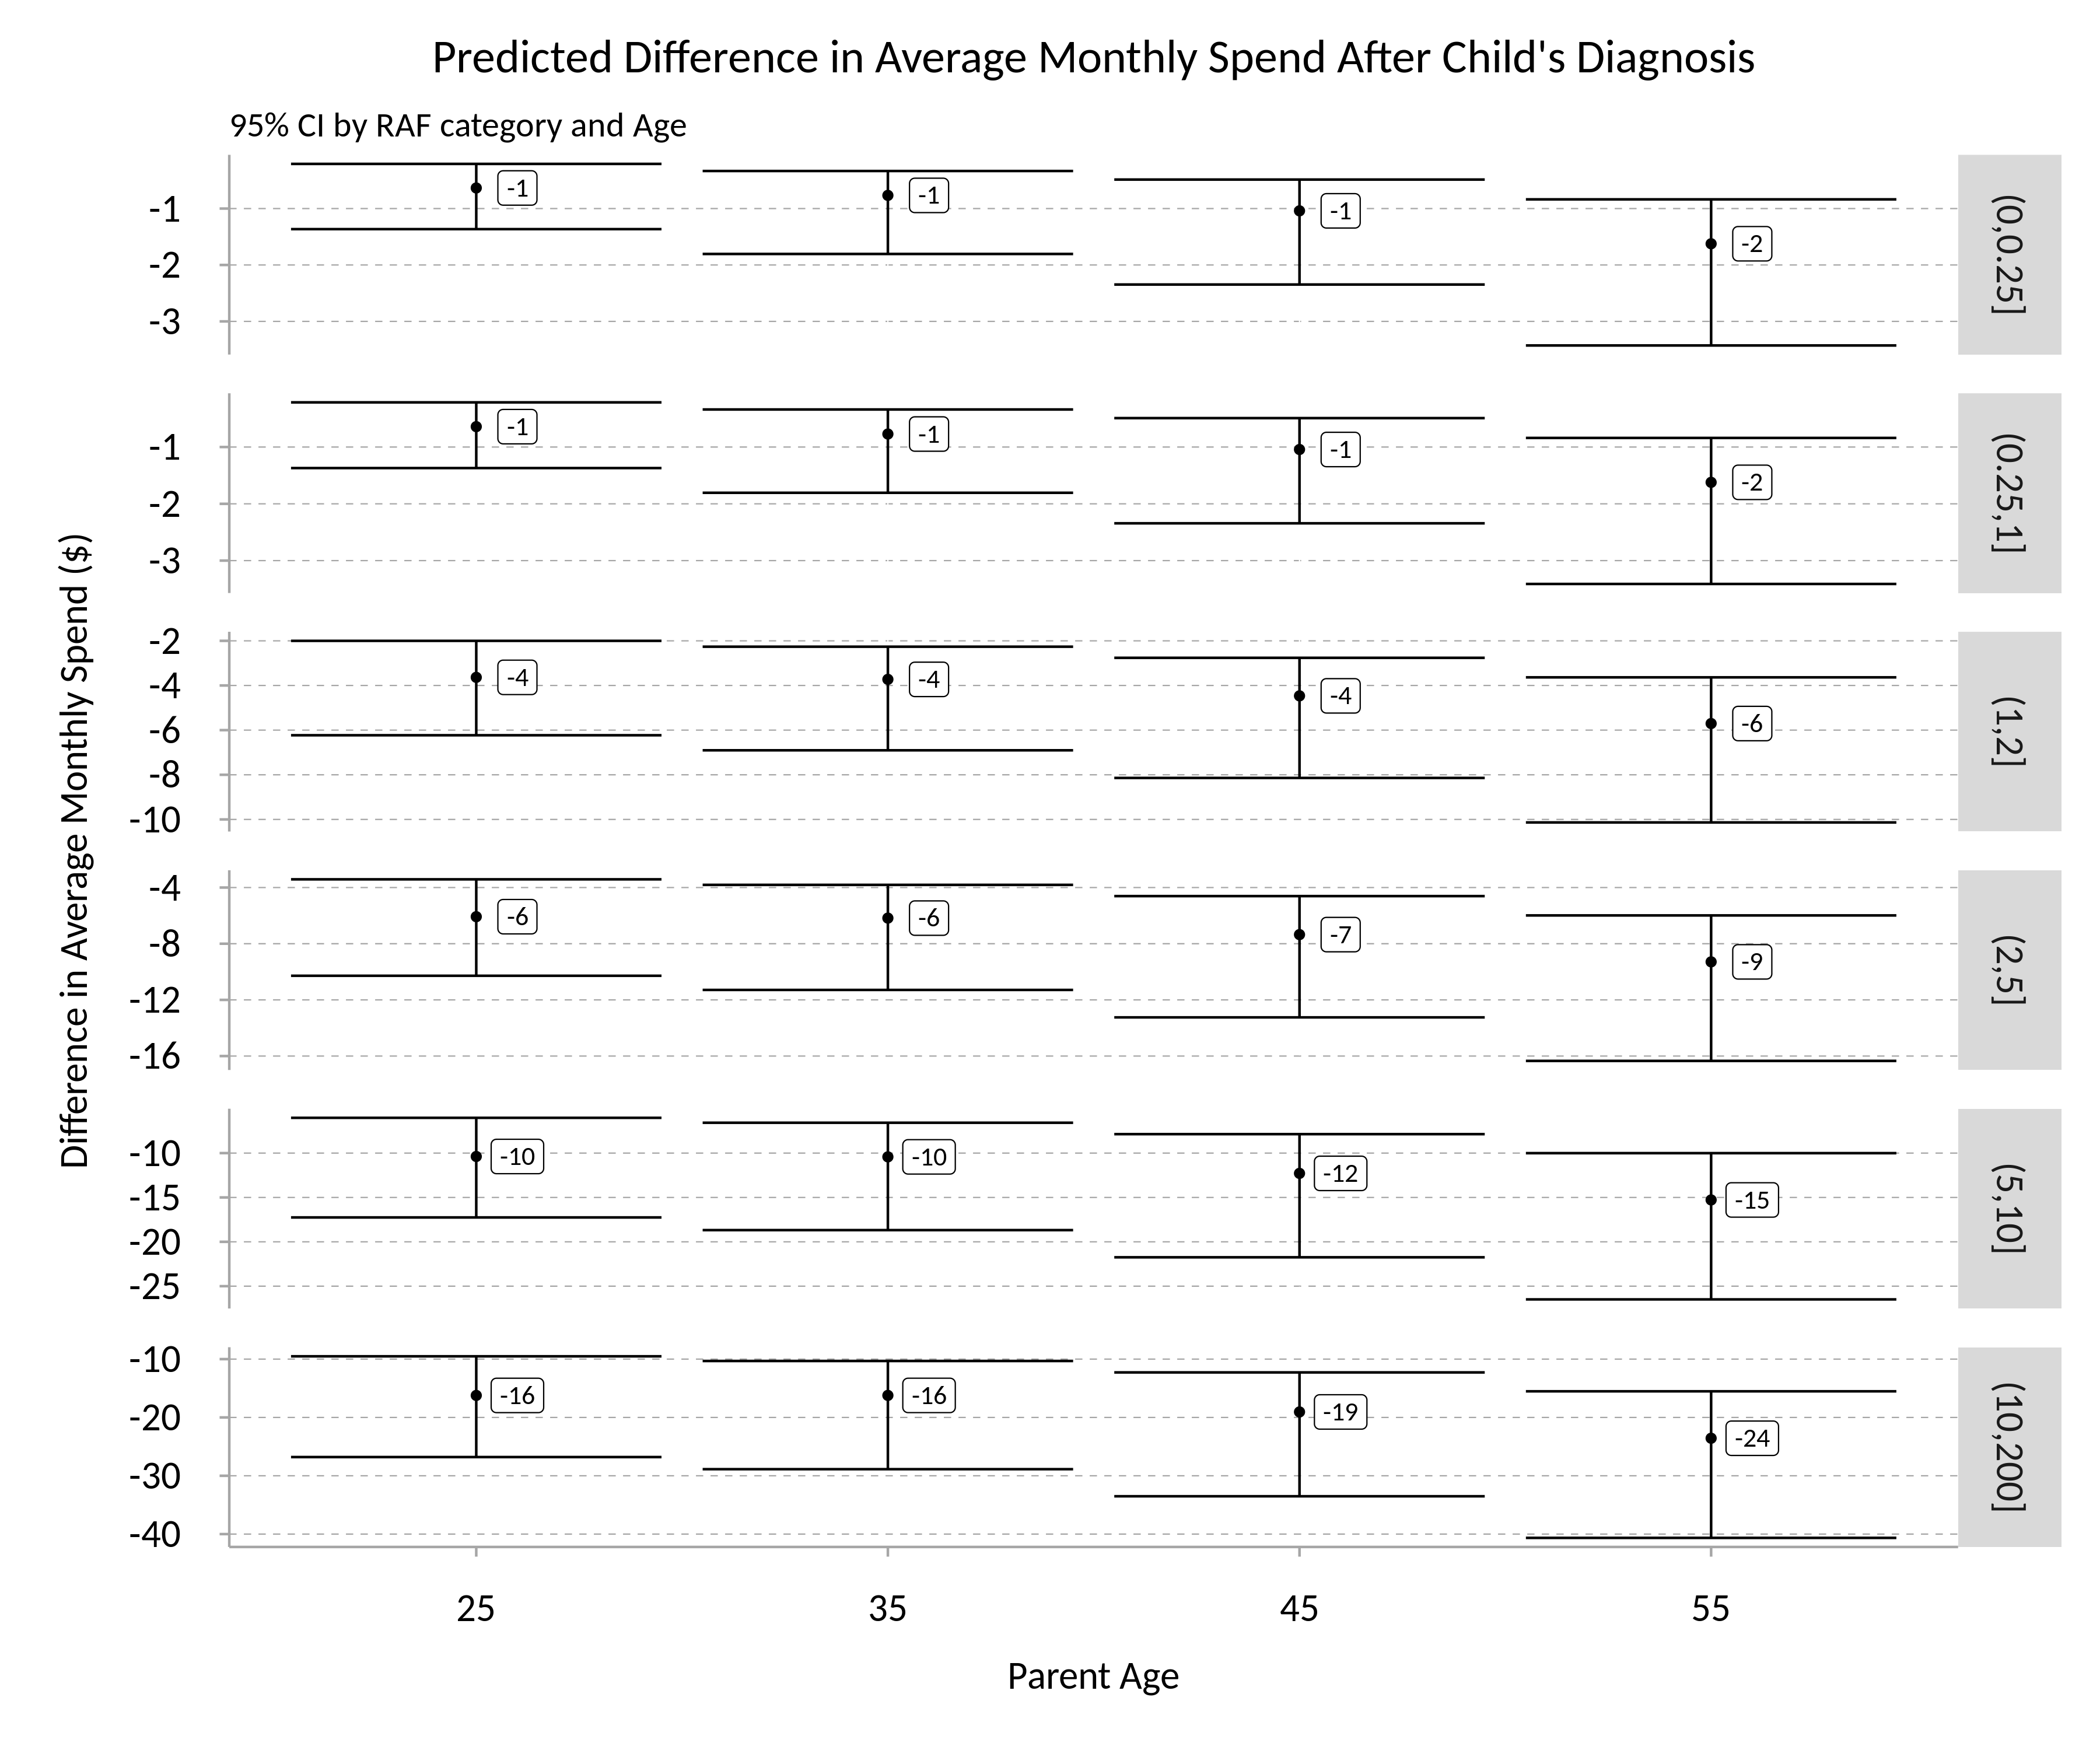
\includegraphics[width=.75\linewidth]{../figures/predicted_spend_female_CA.png}
\end{frame}

\begin{frame}{Trauma effect on men's spending}
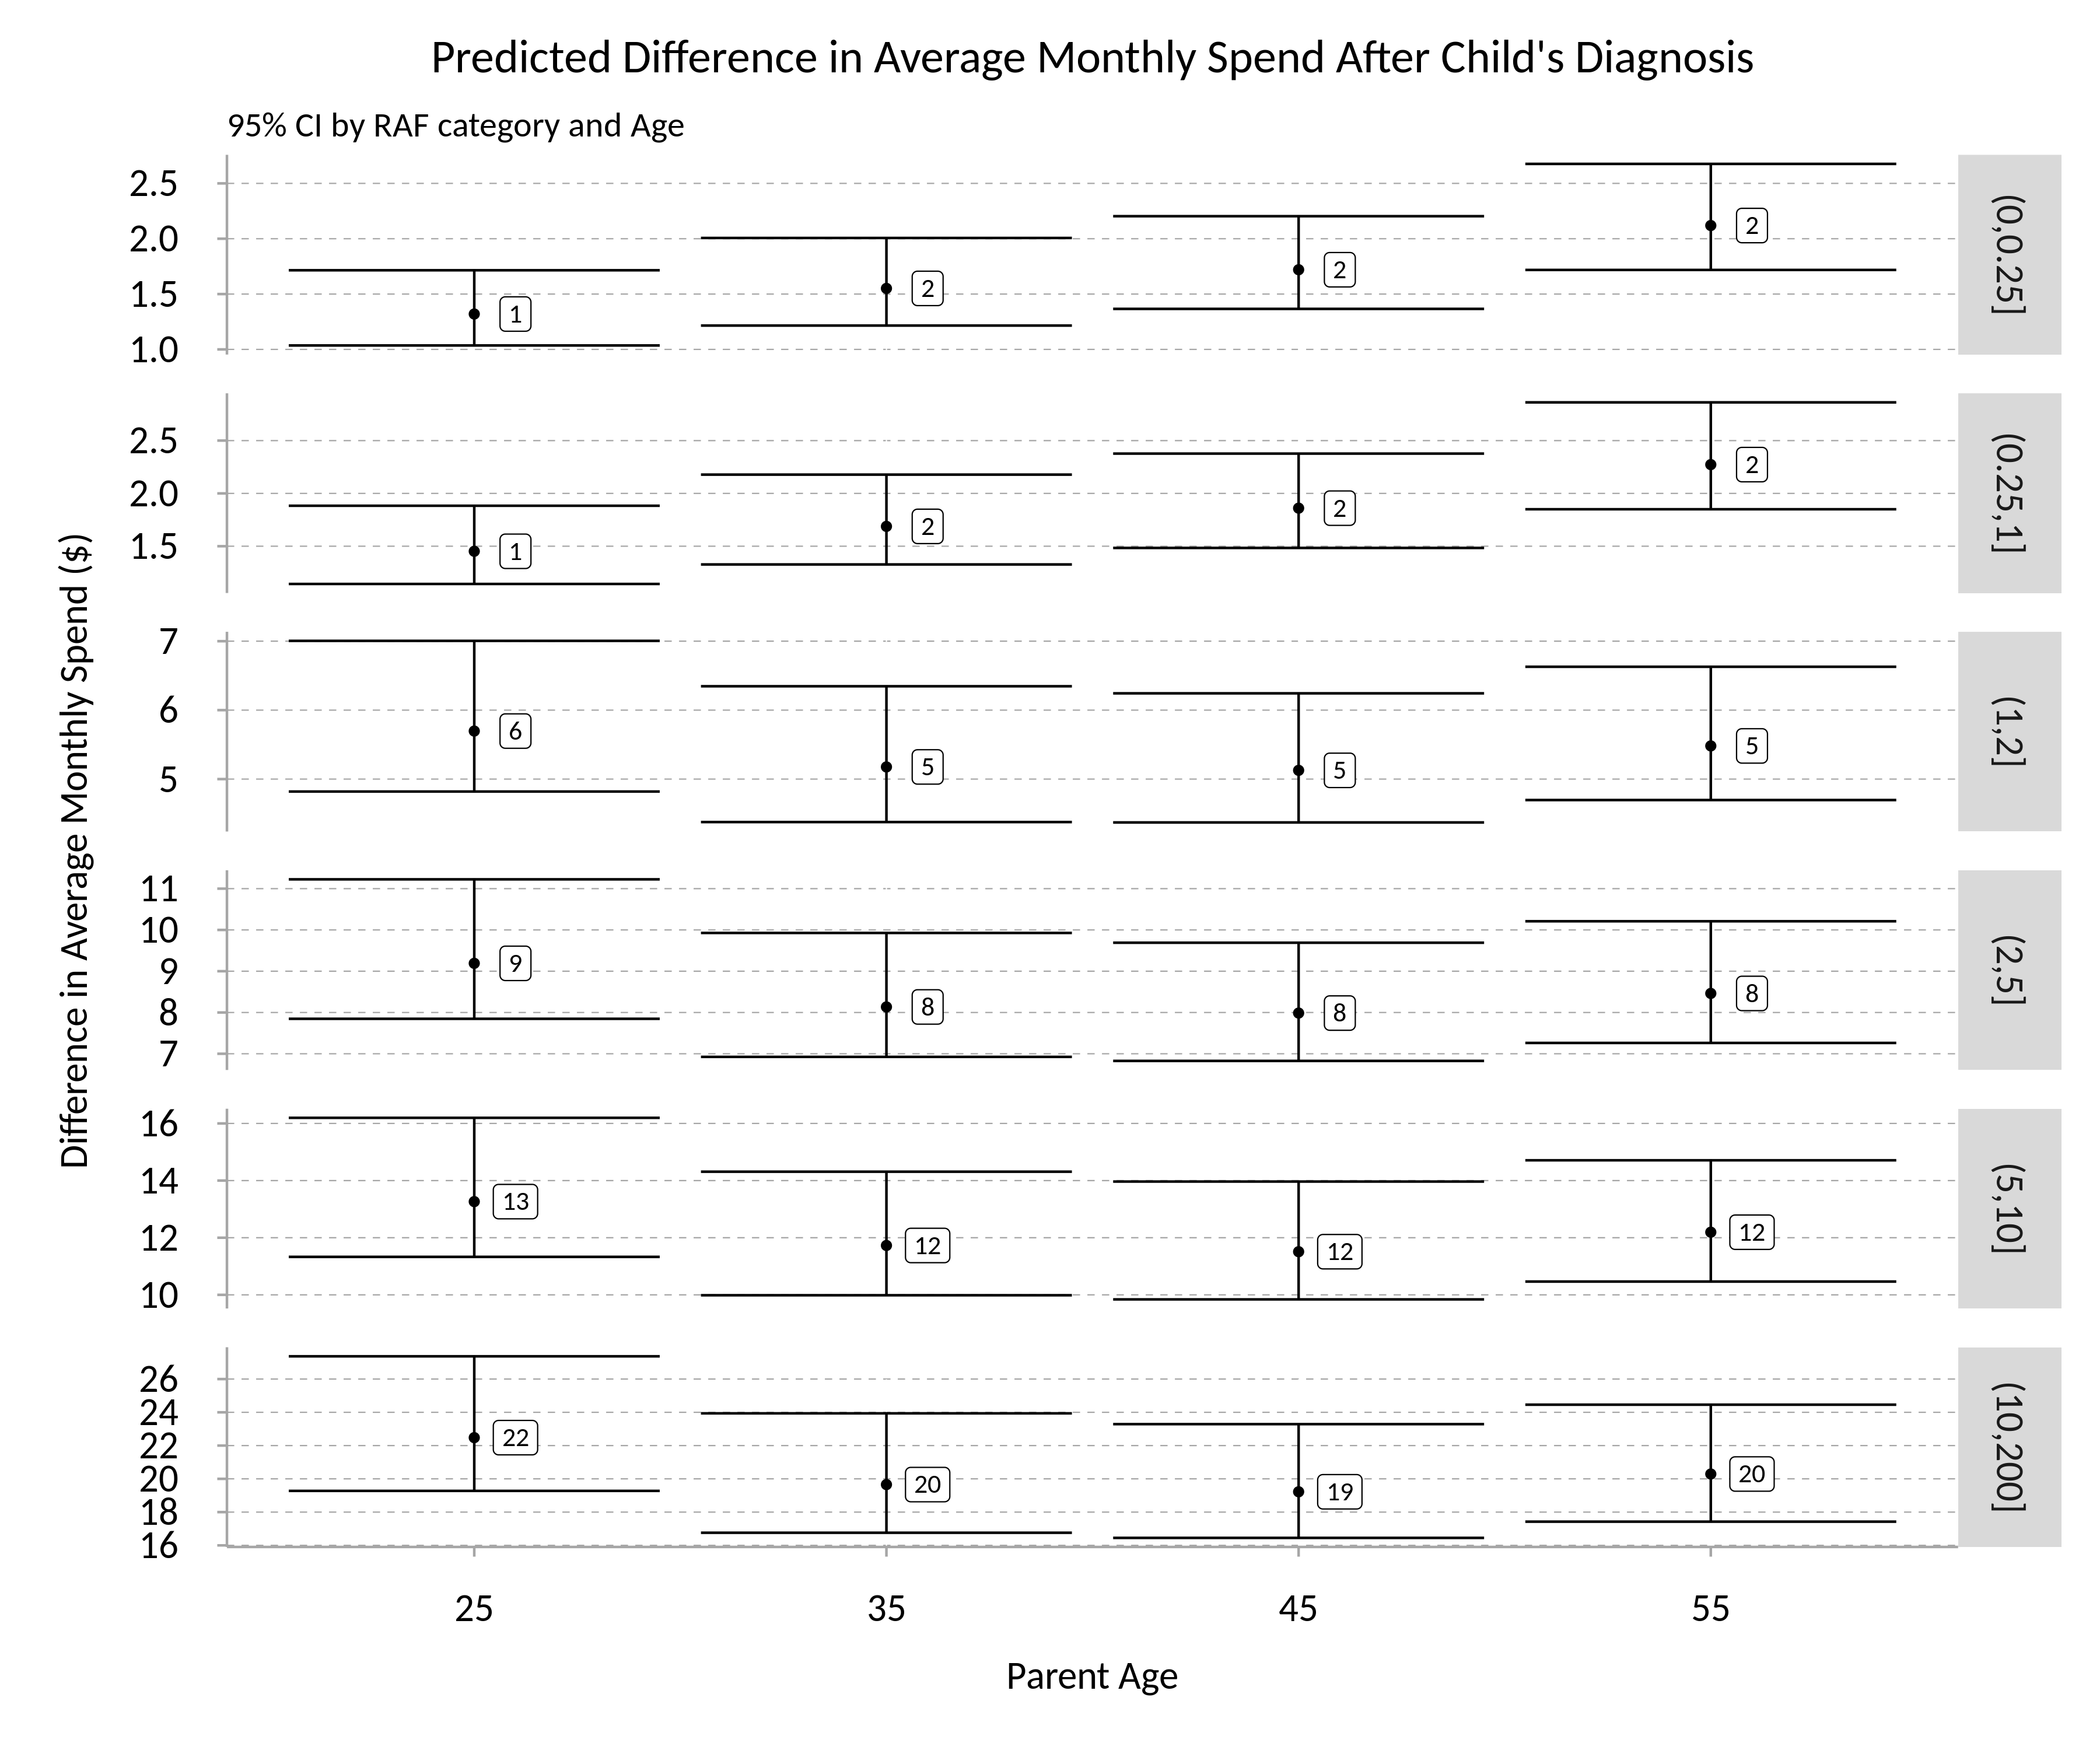
\includegraphics[width=.75\linewidth]{../figures/predicted_spend_male_Trauma.png}
\end{frame}

\begin{frame}{Trauma effect on women's spending}
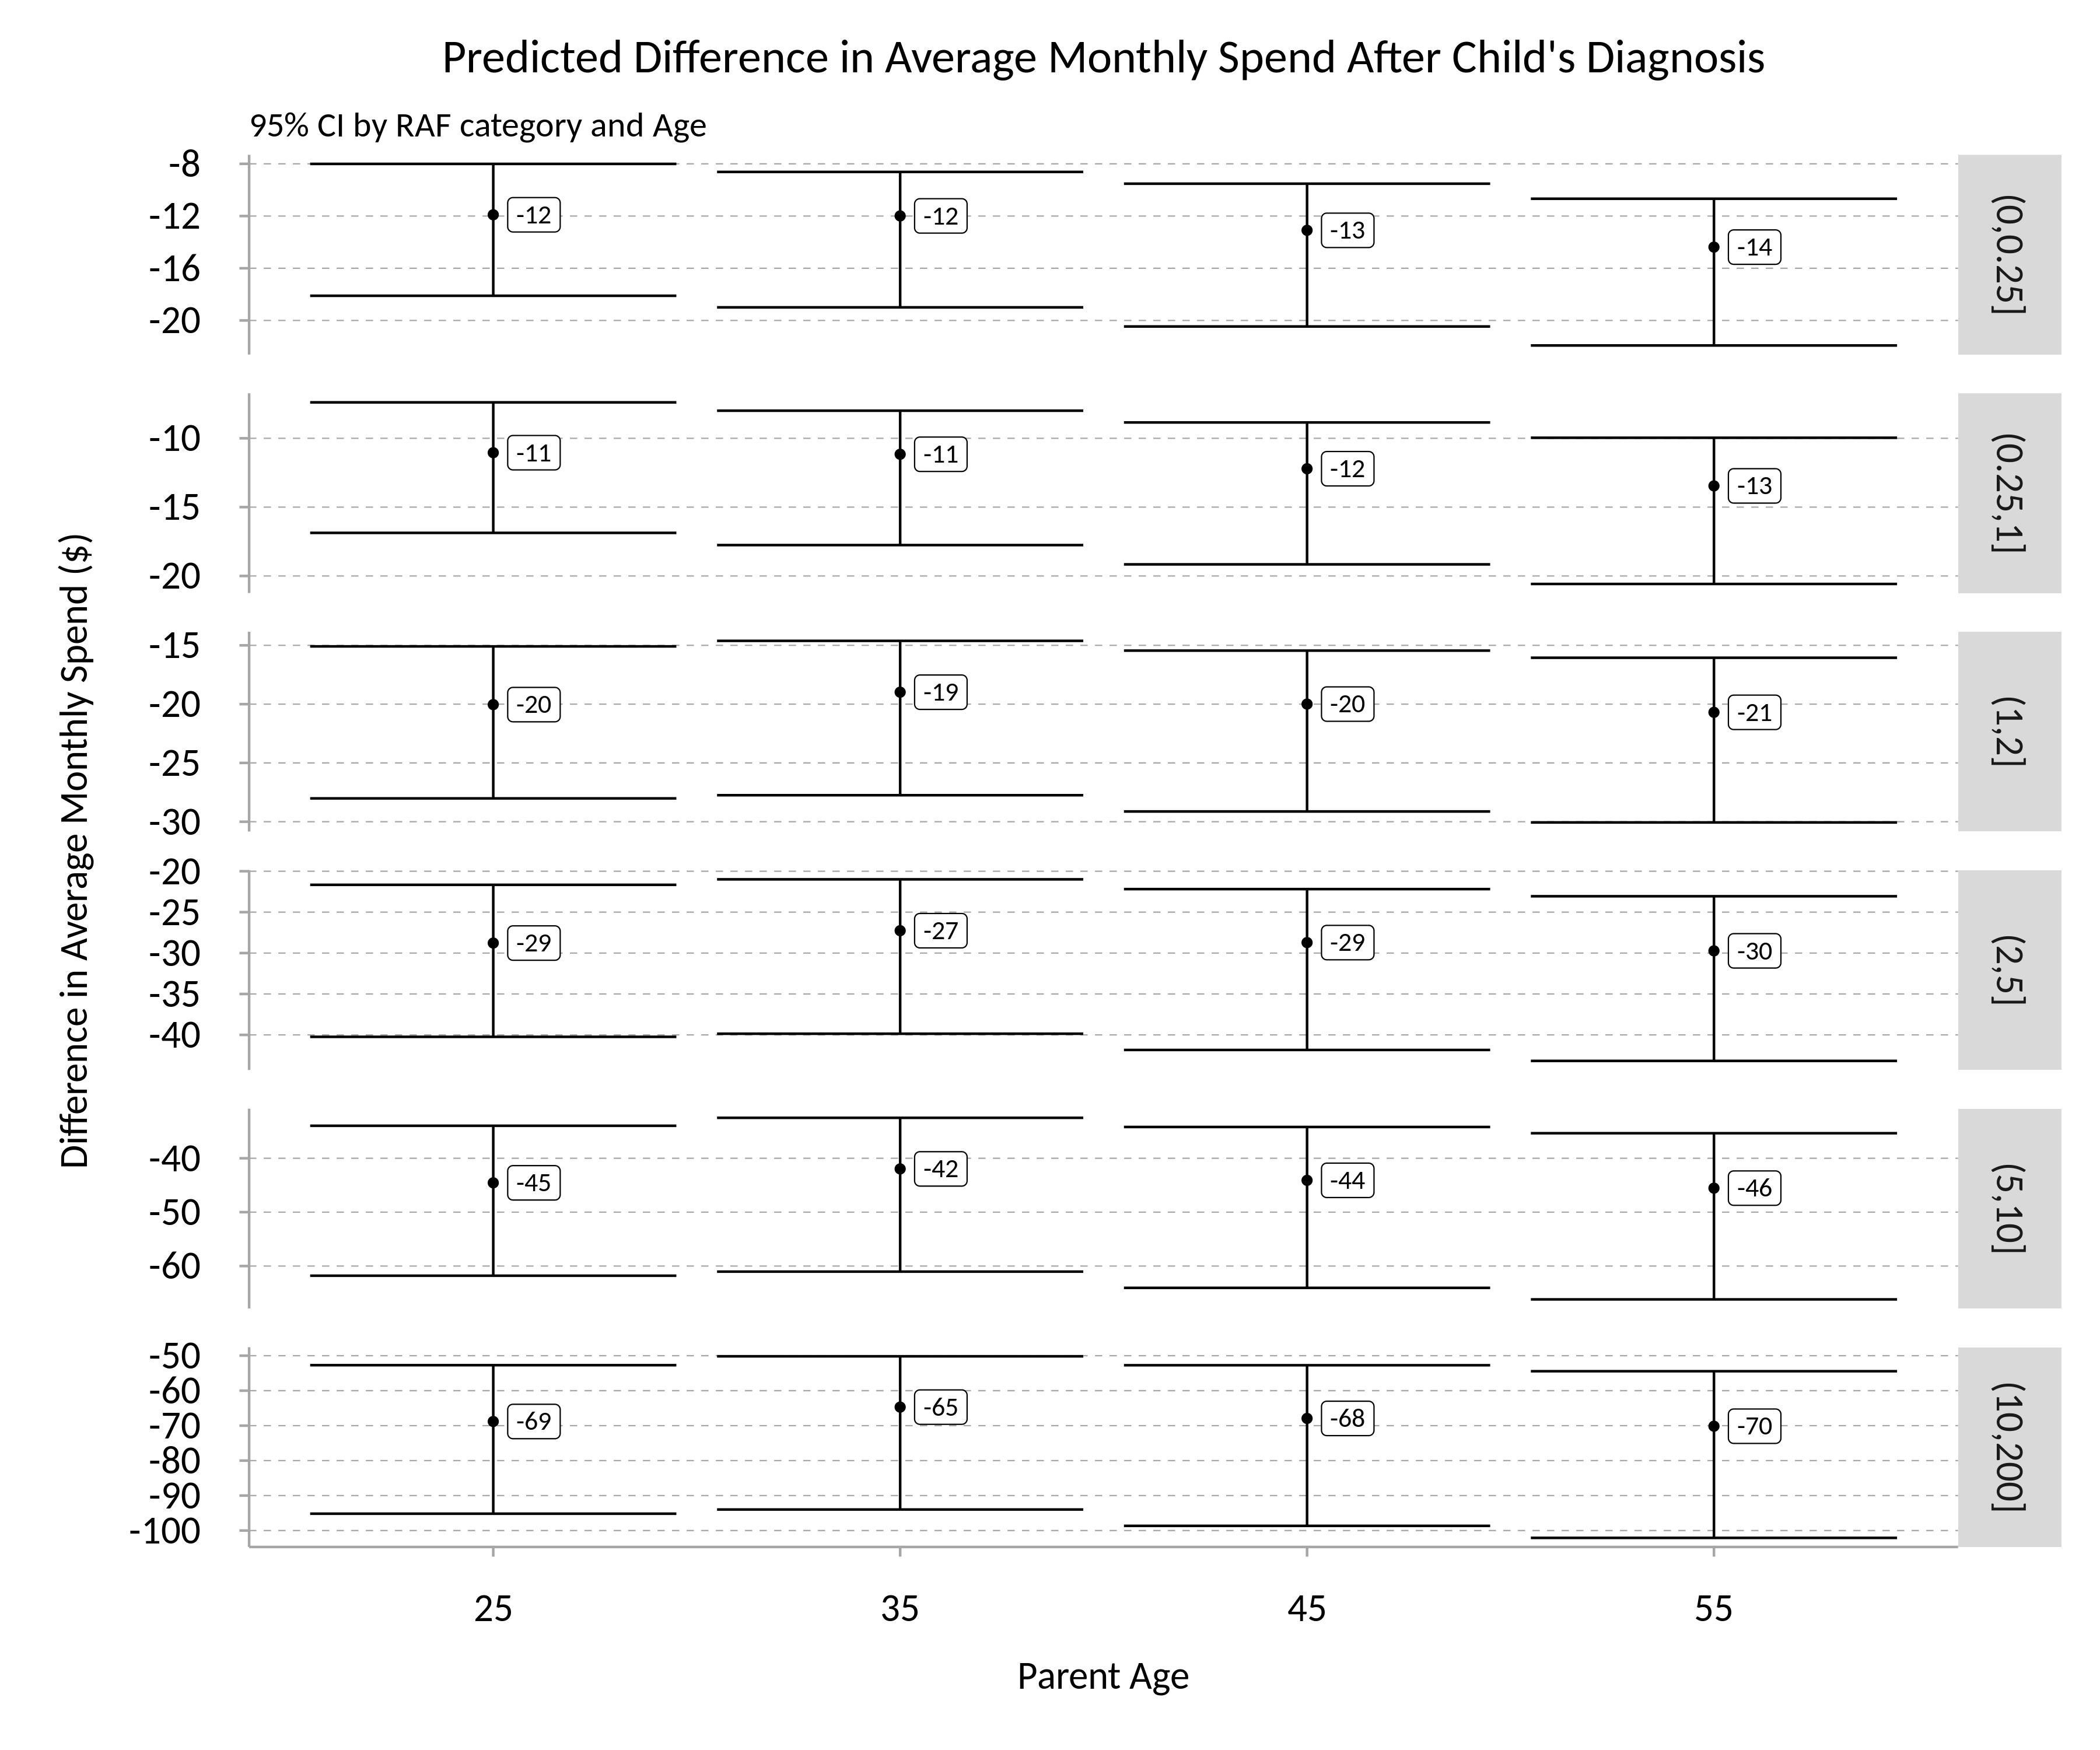
\includegraphics[width=.75\linewidth]{../figures/predicted_spend_female_Trauma.png}
\end{frame}

\begin{frame}{Asthma effect on men's spending}
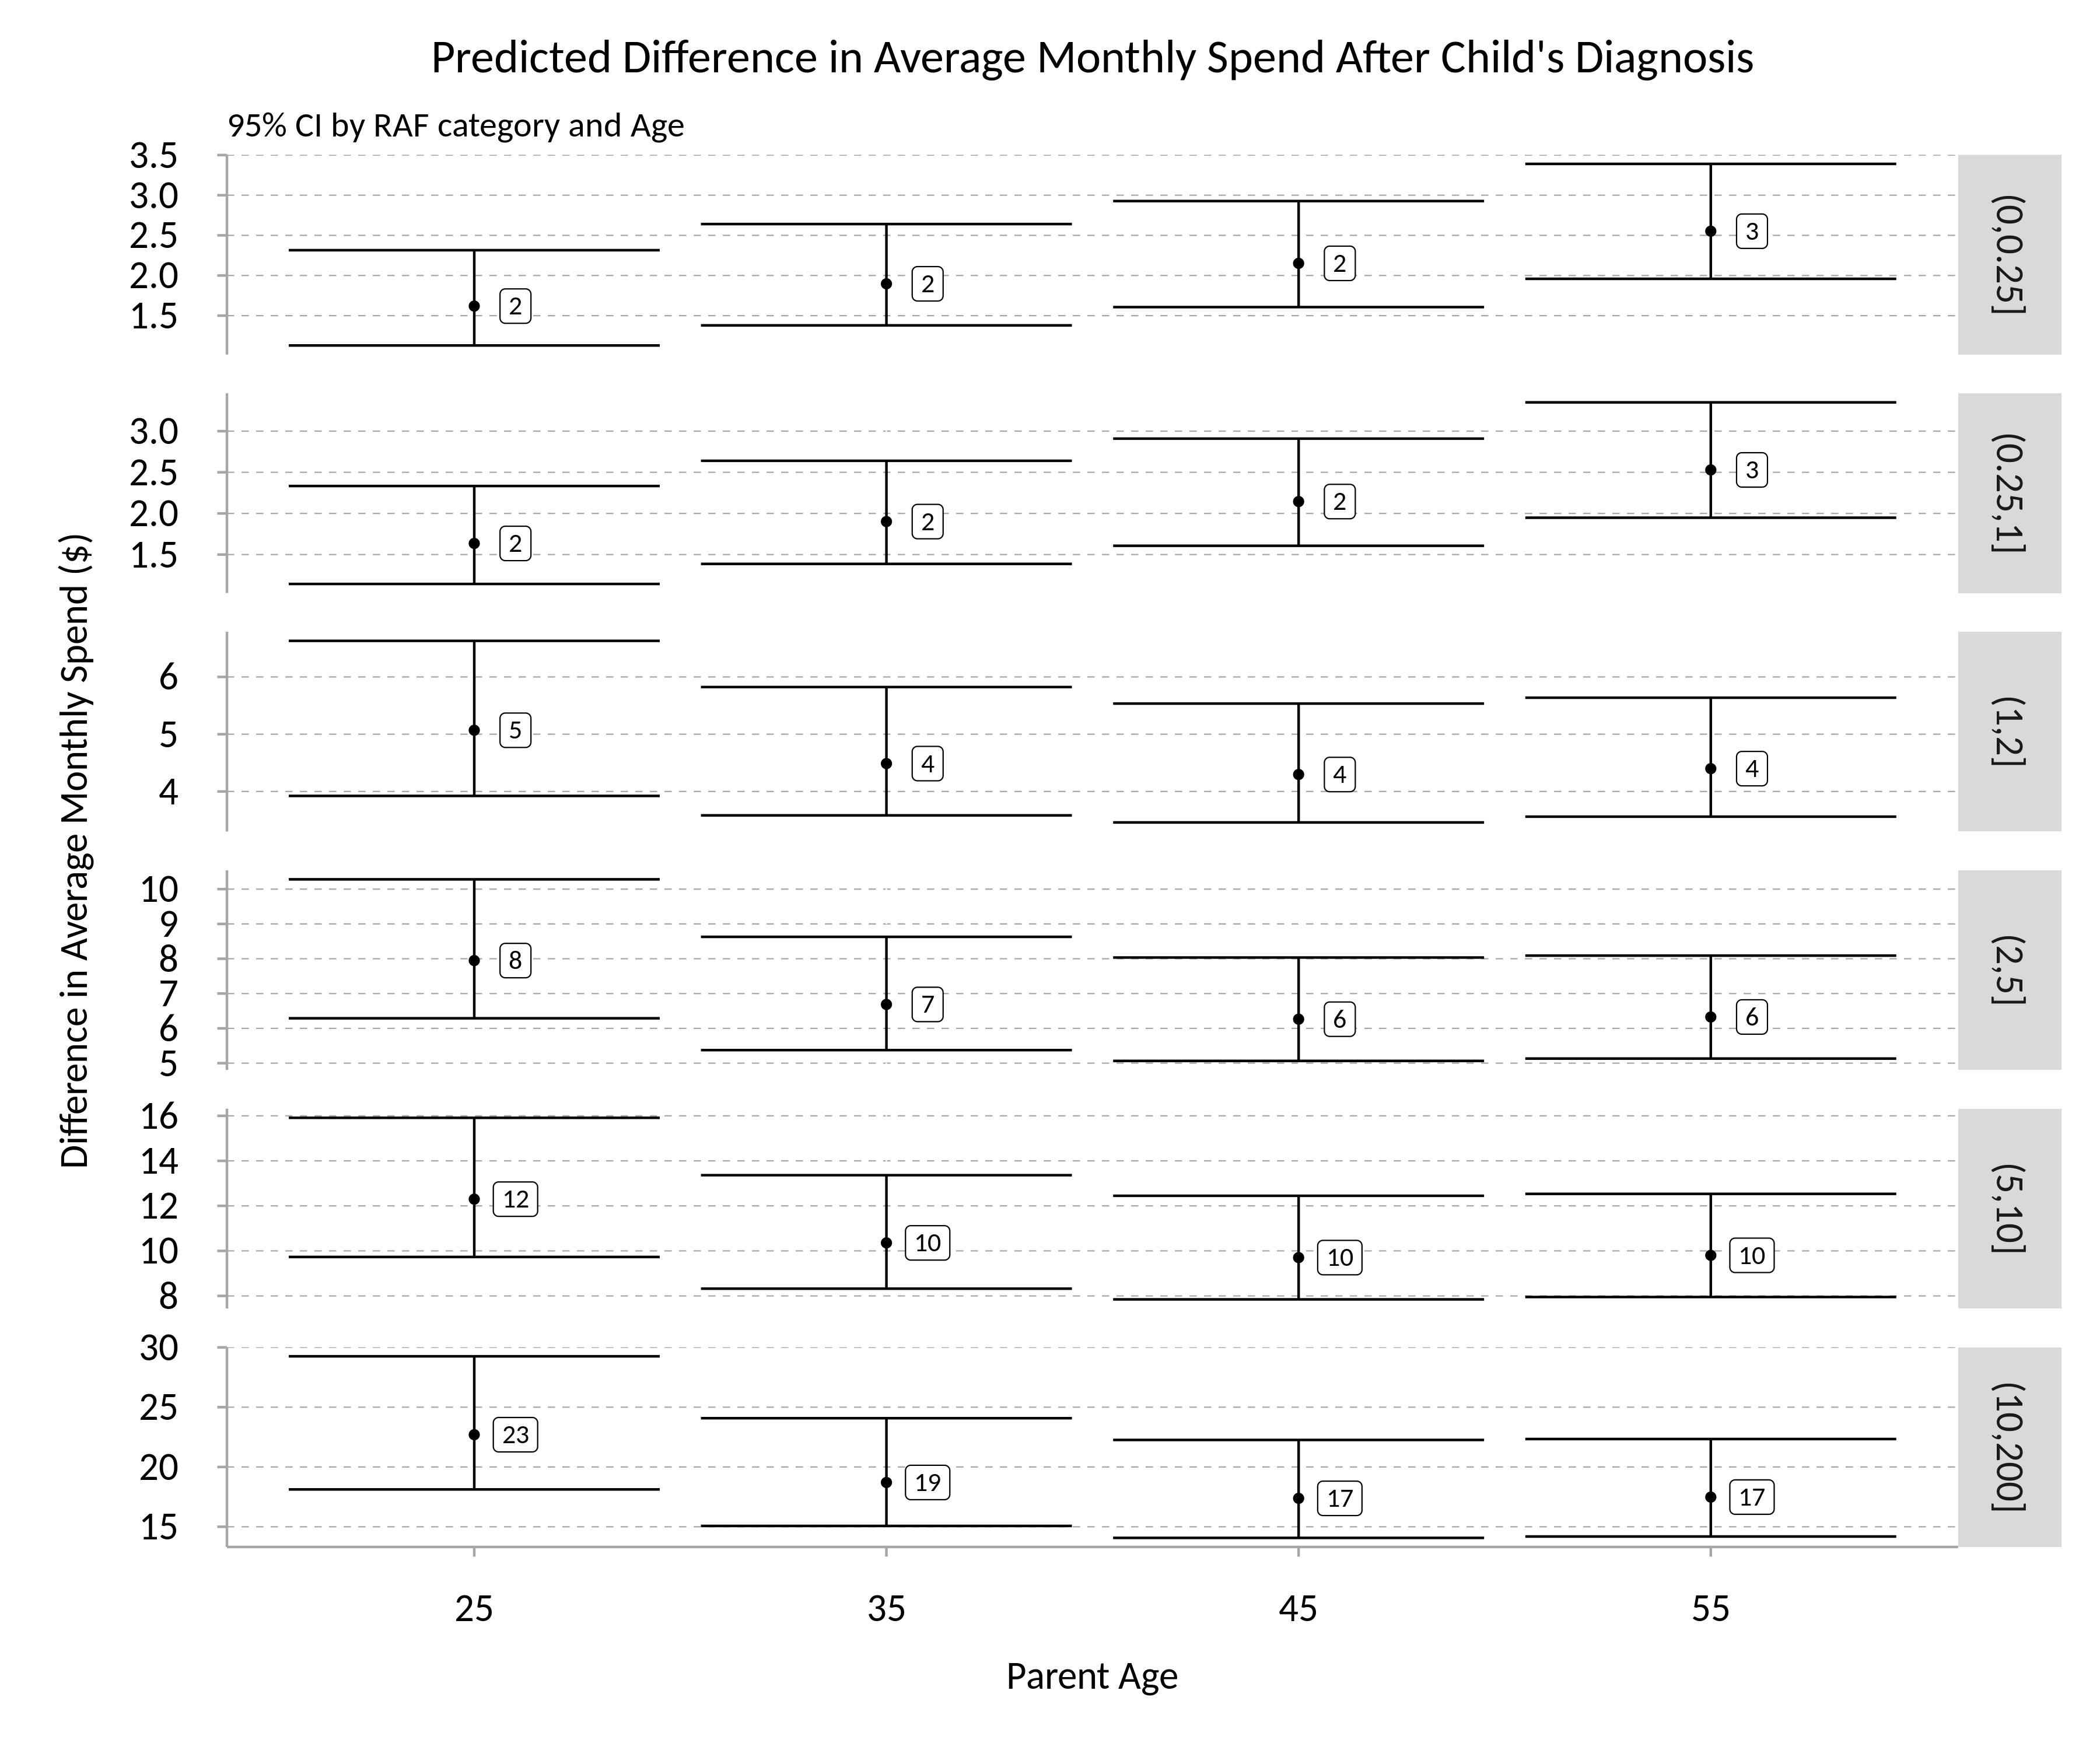
\includegraphics[width=.75\linewidth]{../figures/predicted_spend_male_Asthma.png}
\end{frame}

\begin{frame}{Asthma effect on women's spending}
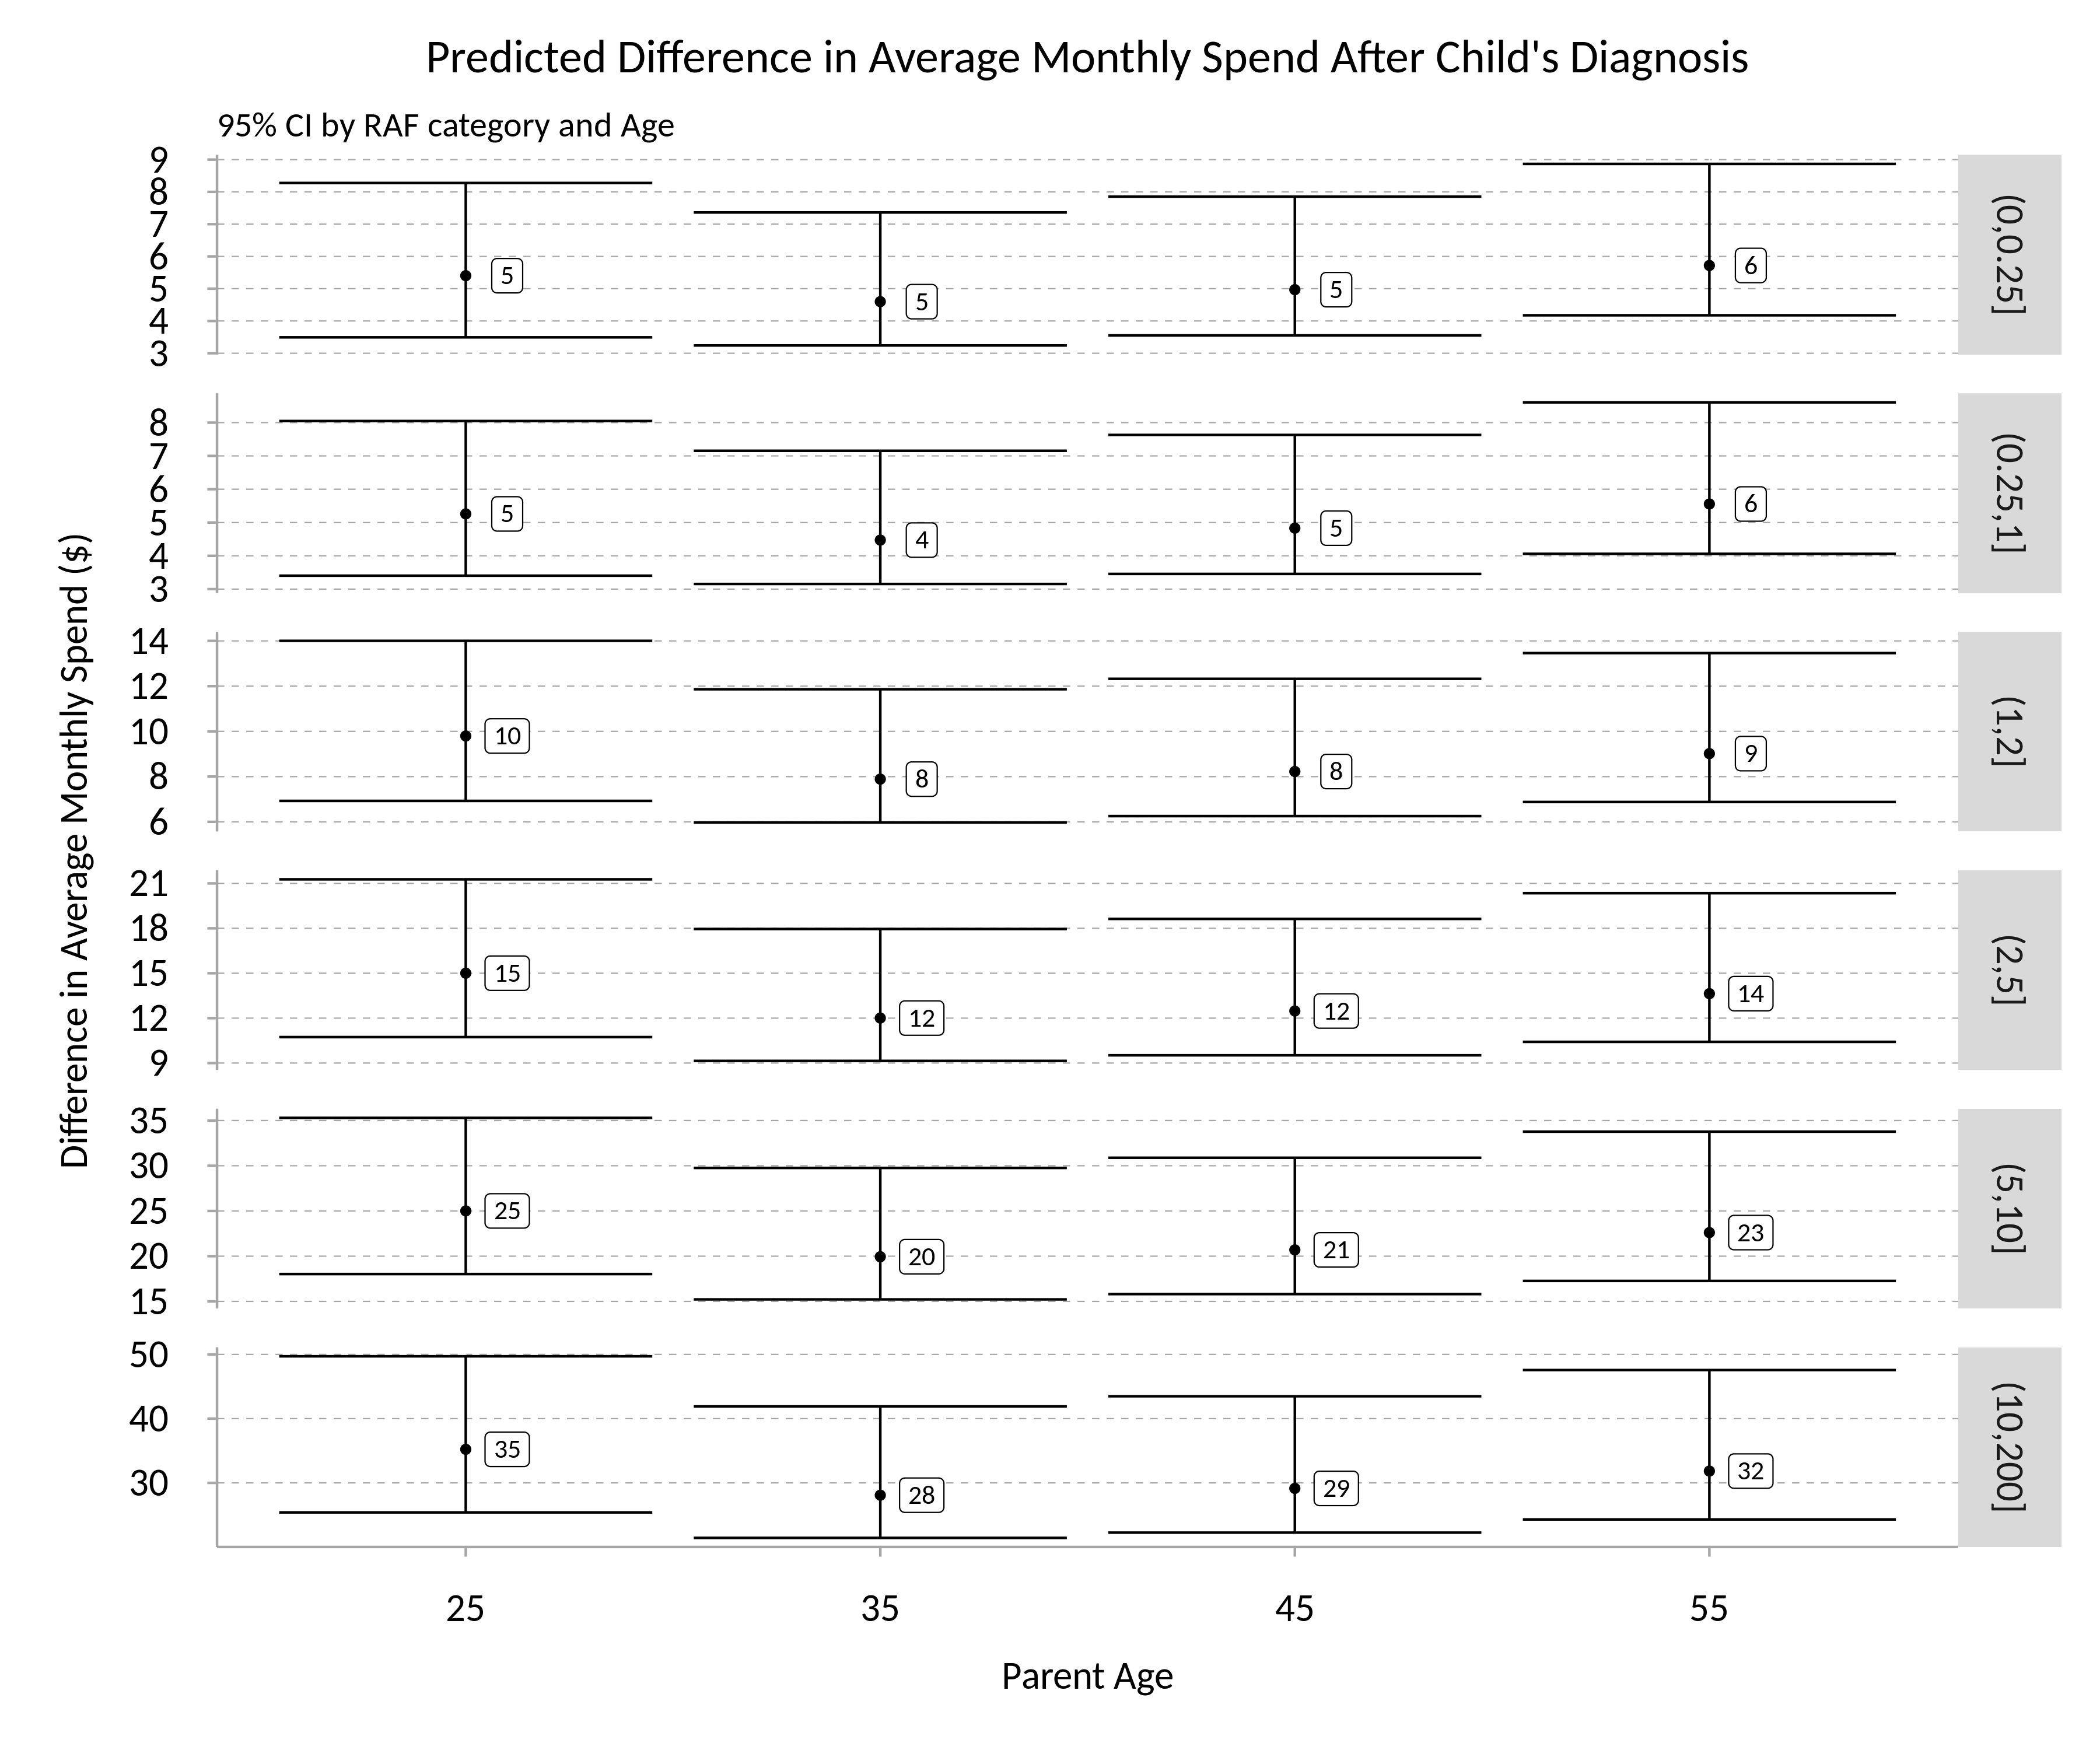
\includegraphics[width=.75\linewidth]{../figures/predicted_spend_female_Asthma.png}
\end{frame}

\begin{frame}{T1D effect on men's spending}
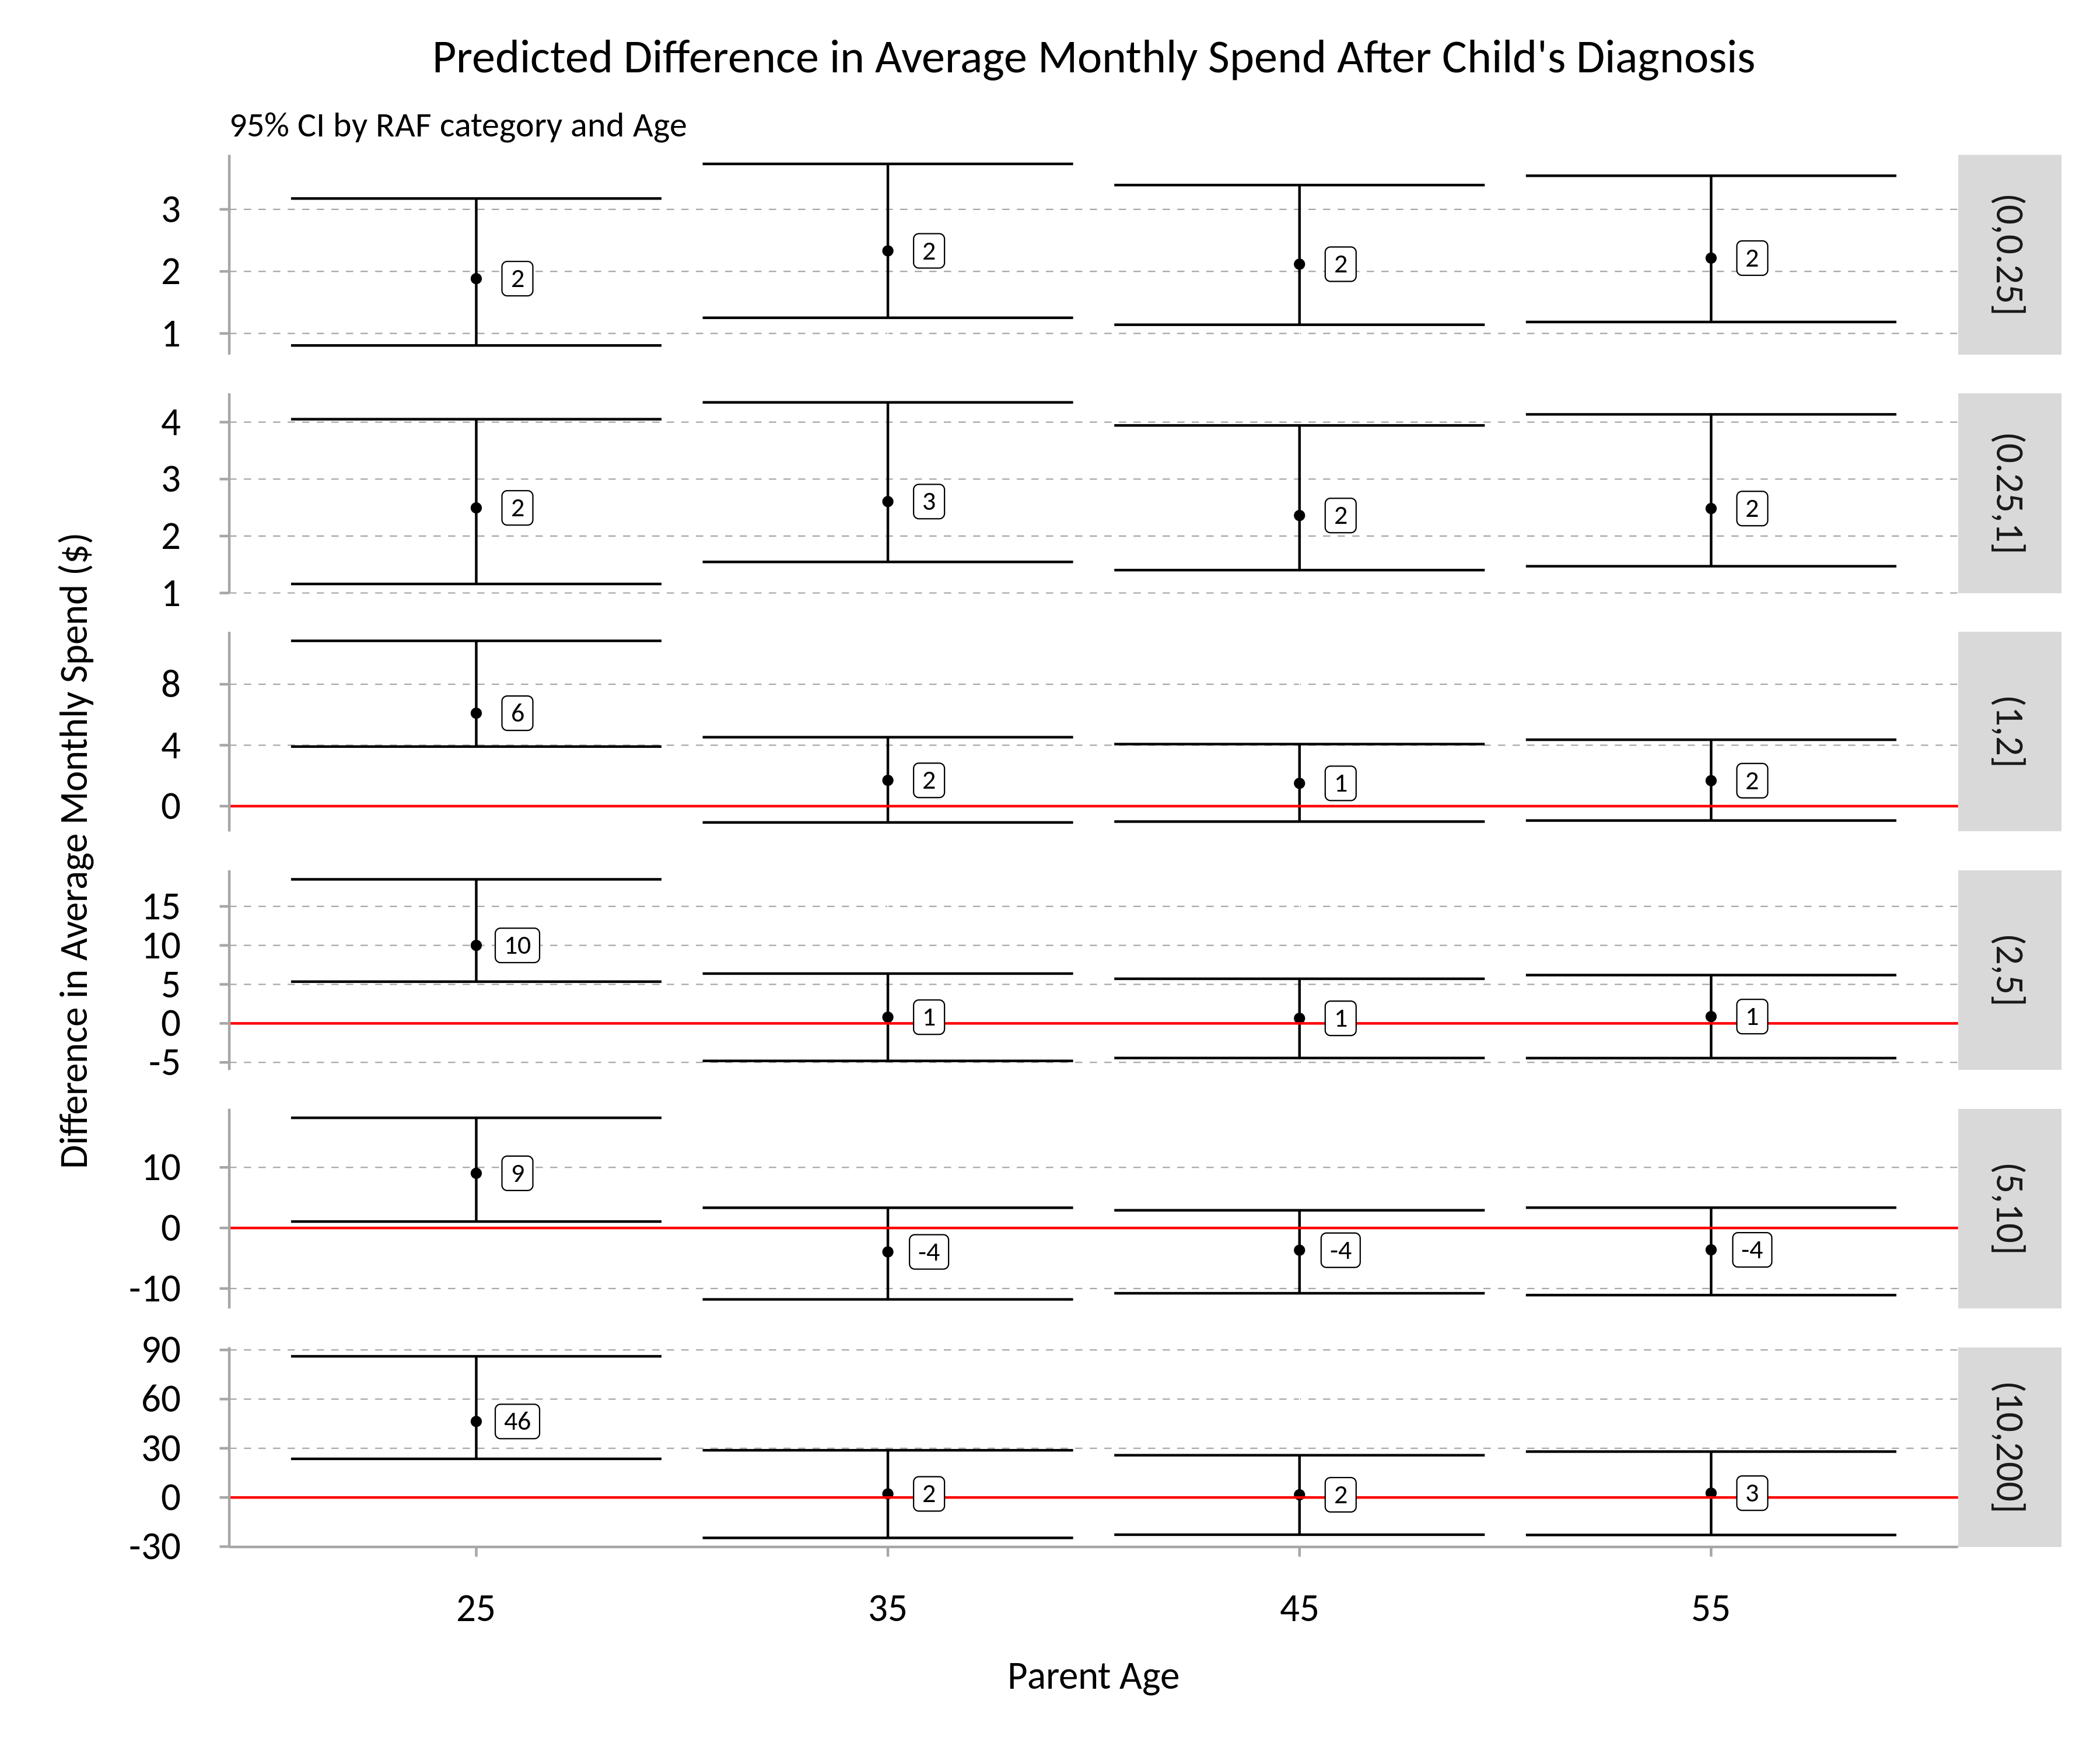
\includegraphics[width=.75\linewidth]{../figures/predicted_spend_male_T1D.png}
\end{frame}

\begin{frame}{T1D effect on women's spending}
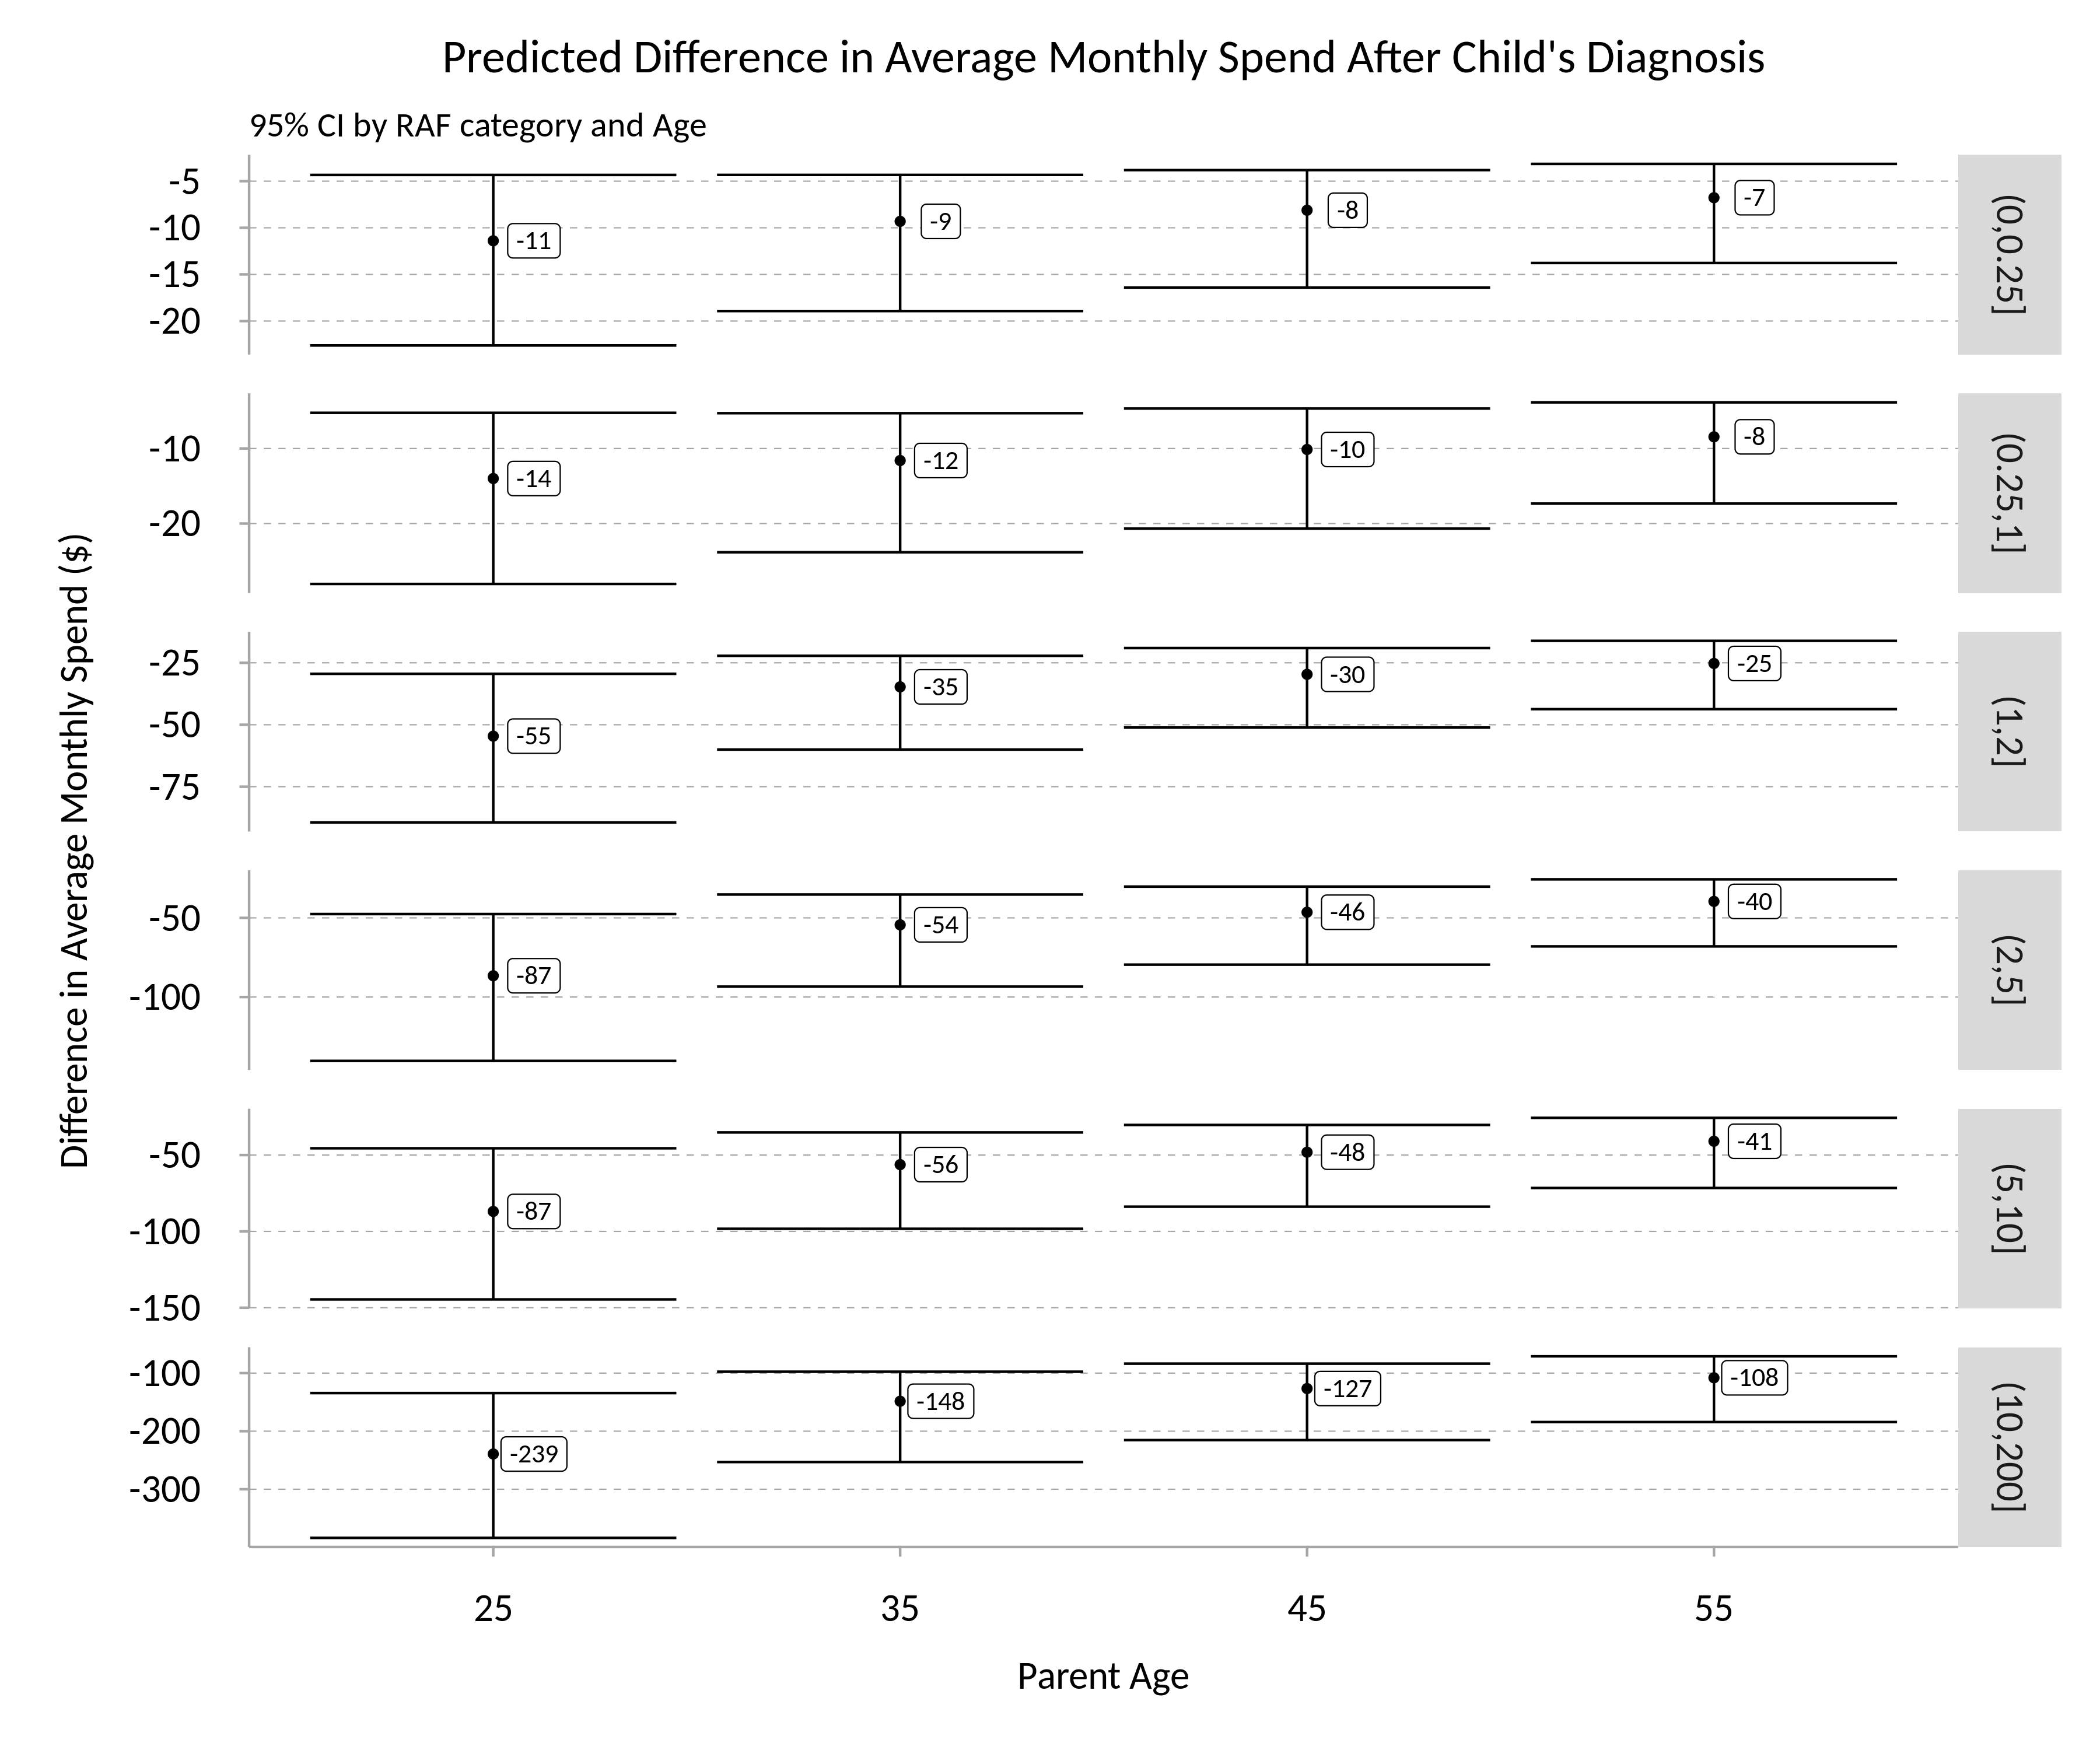
\includegraphics[width=.75\linewidth]{../figures/predicted_spend_female_T1D.png}
\end{frame}

\begin{frame}{T1D effect on women's spending}
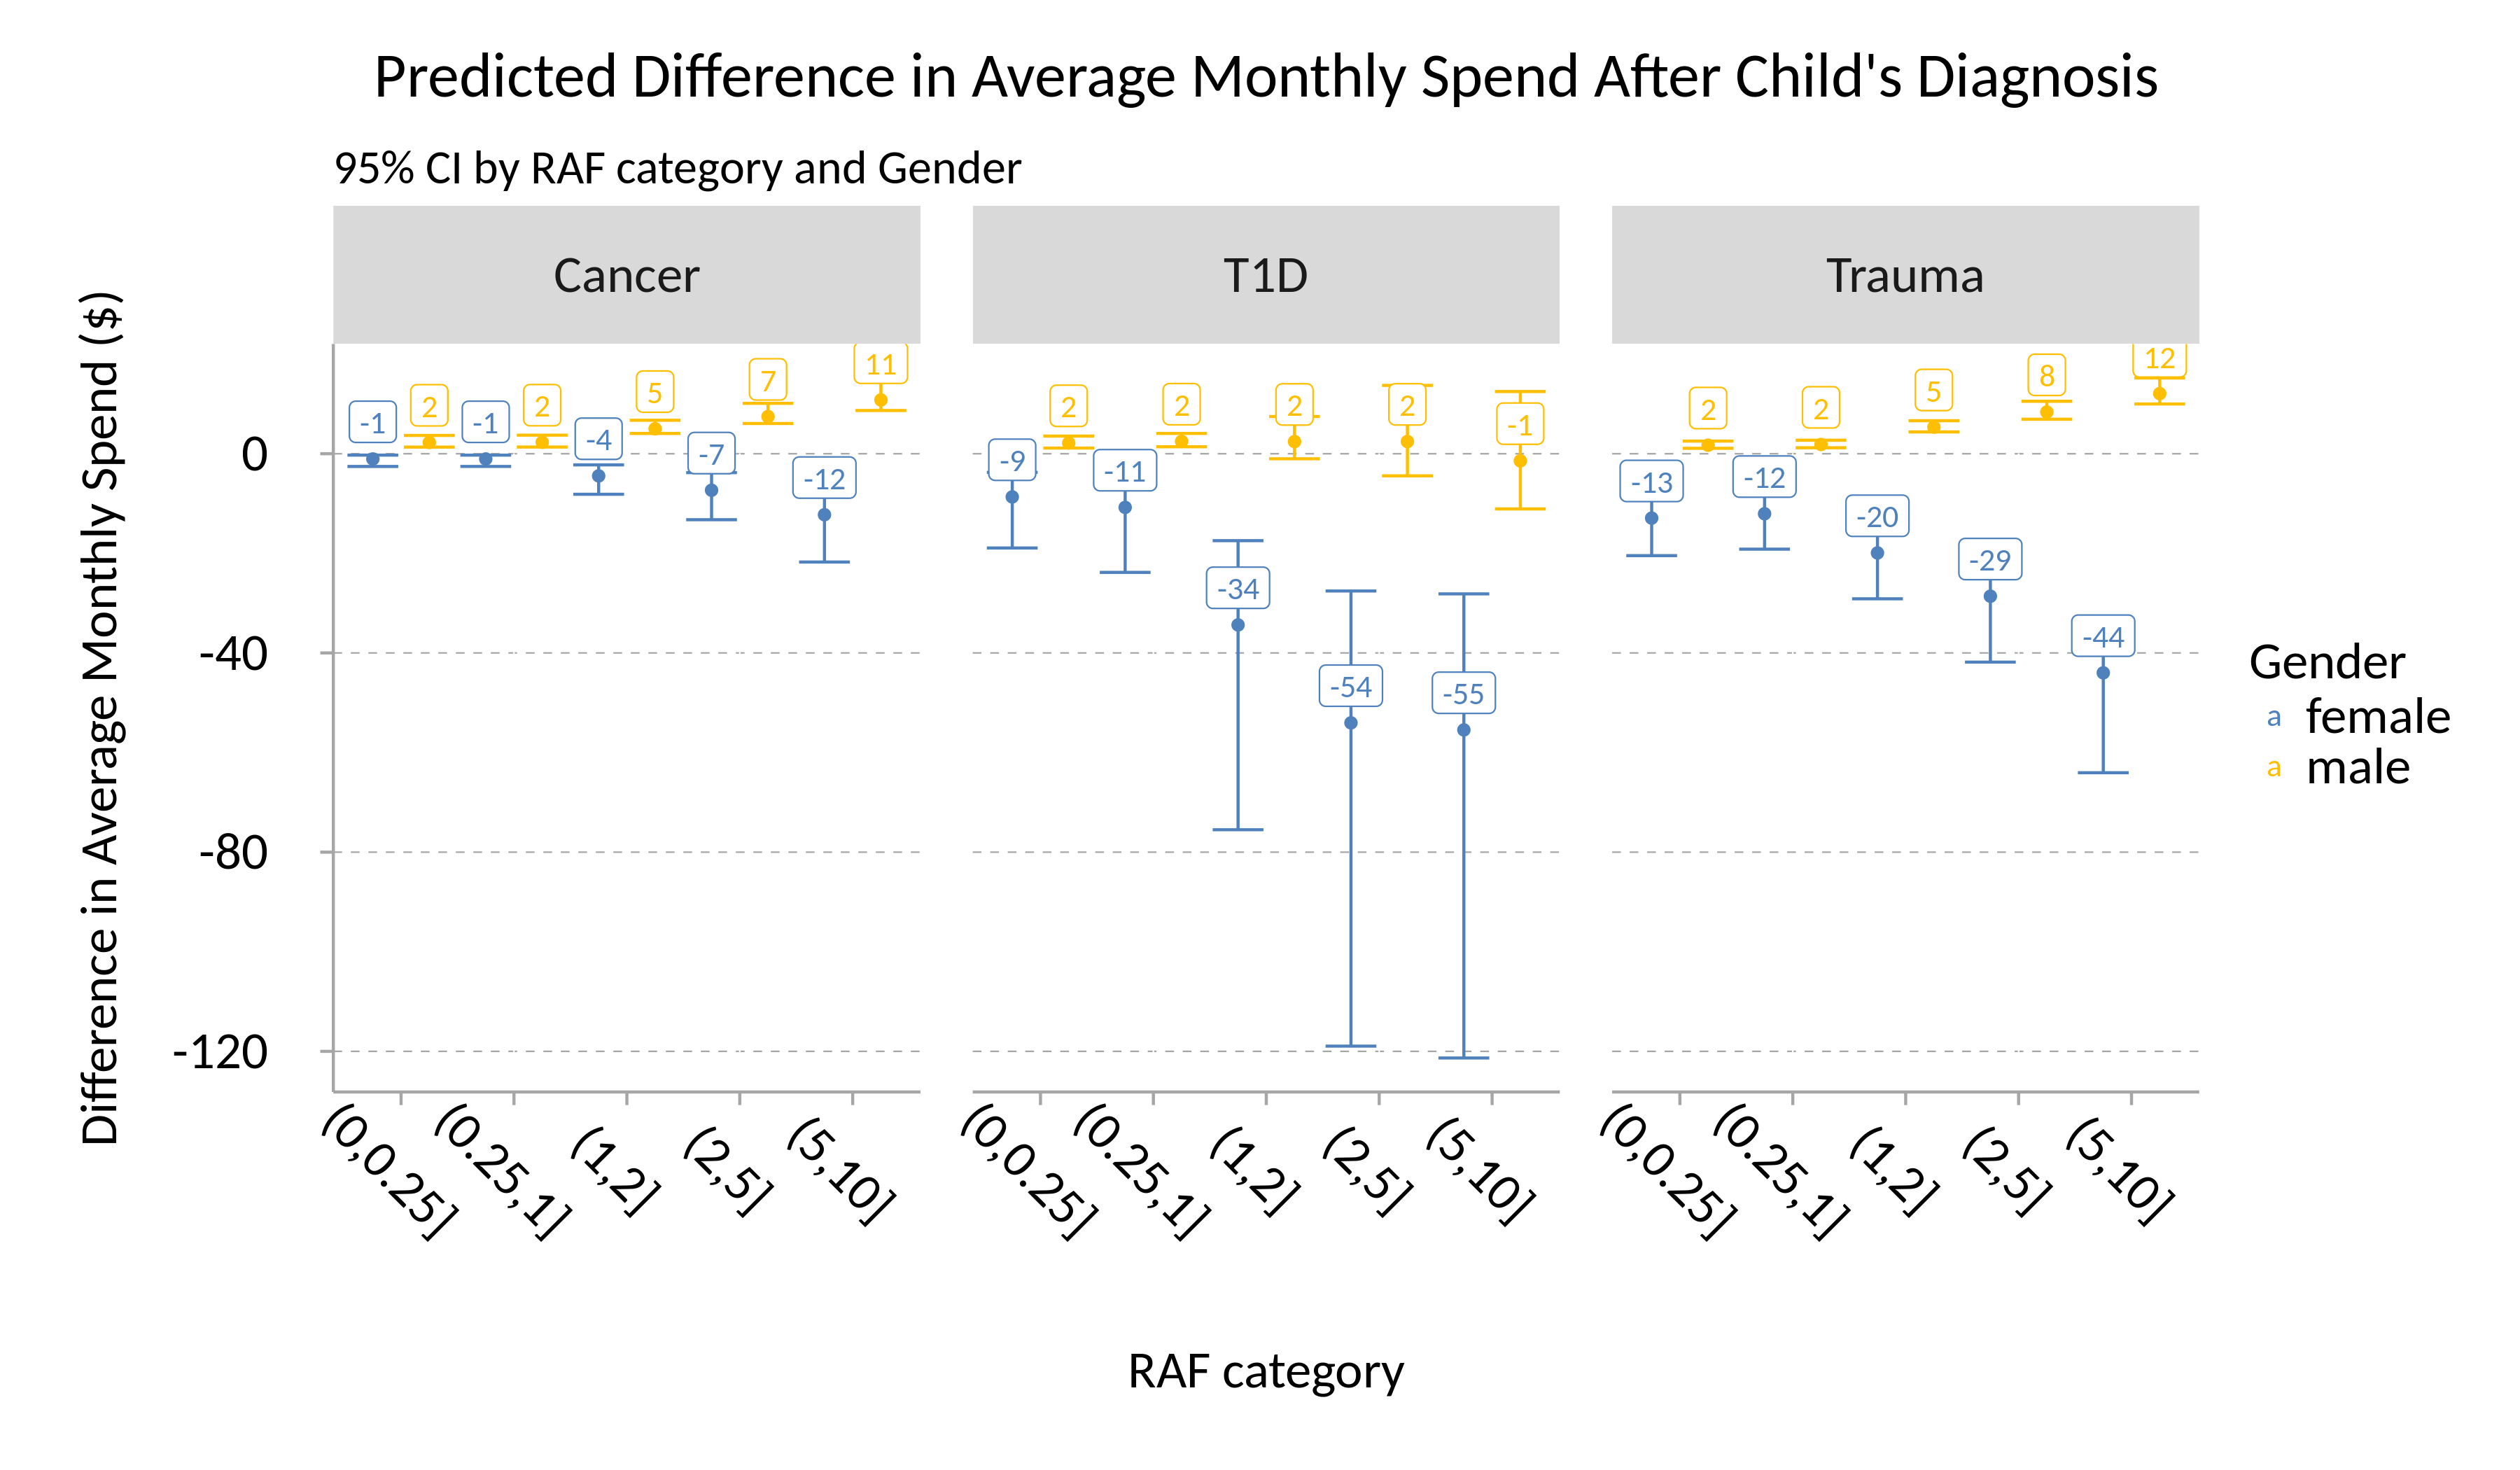
\includegraphics[width=\linewidth]{../figures/spend_diff_Cancer_T1D.png}
\end{frame}

\begin{frame}
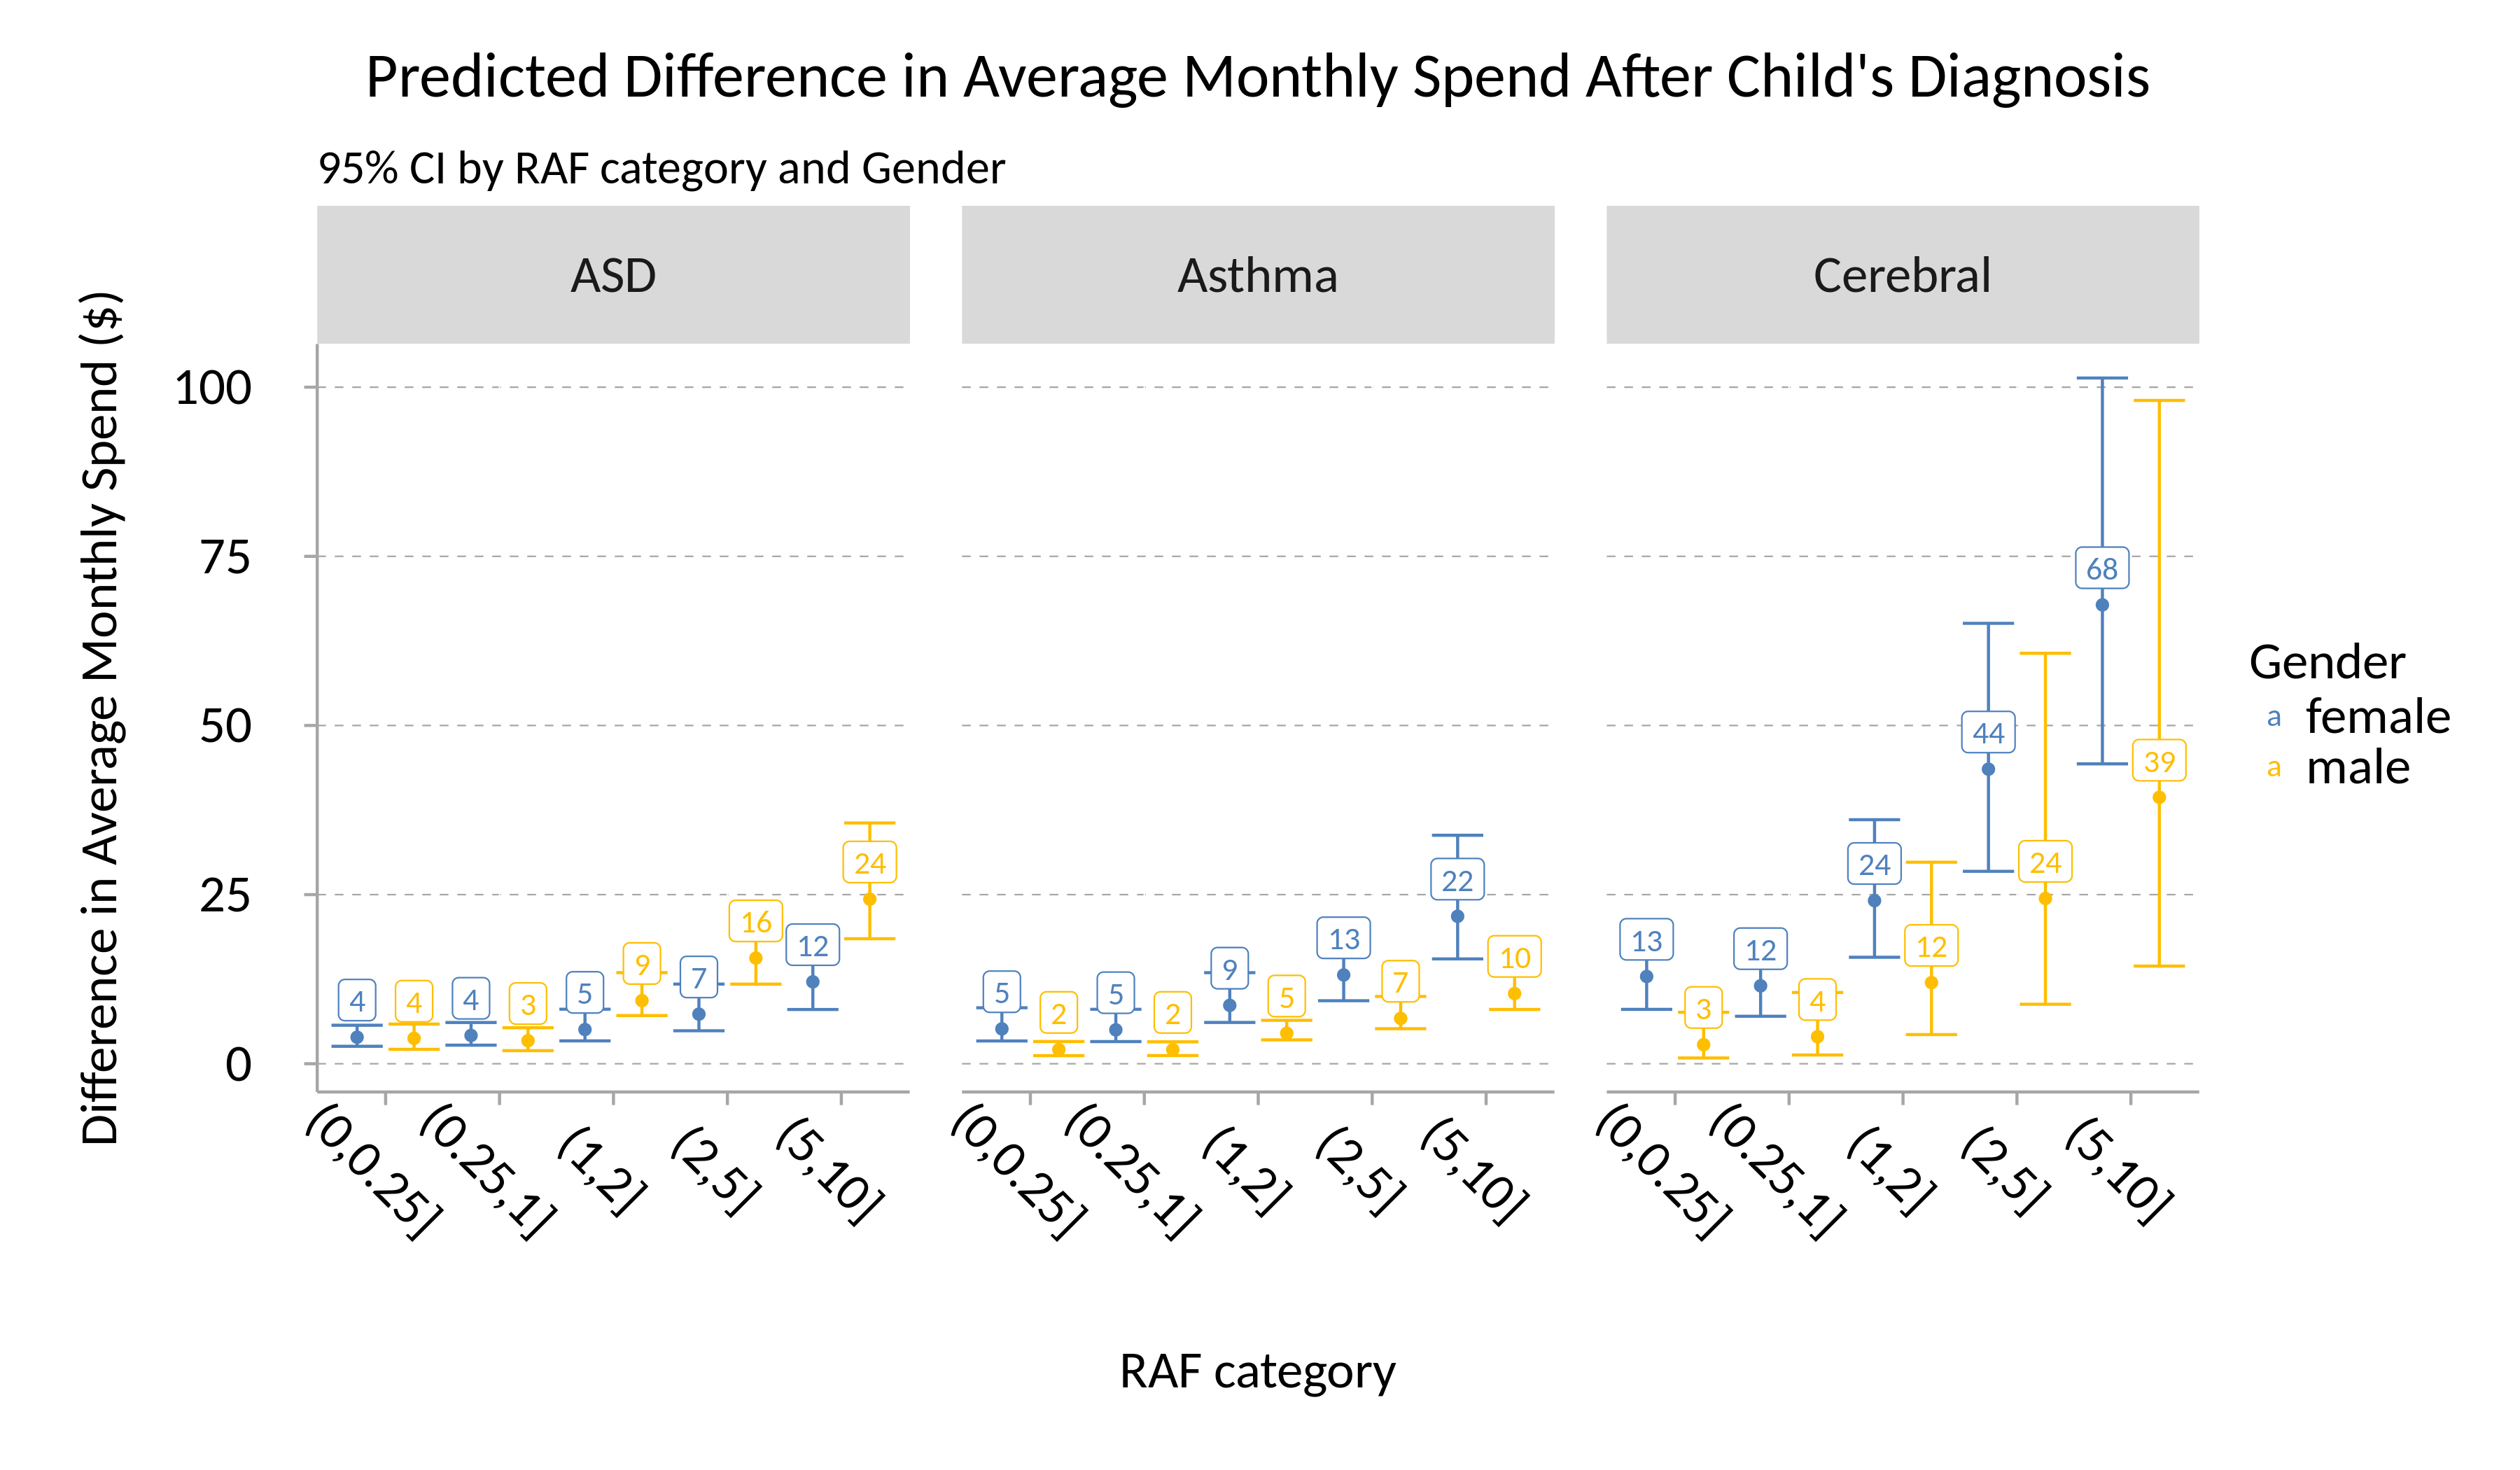
\includegraphics[width=\linewidth]{../figures/spend_diff_ASD_Cerebral.png}
\end{frame}

\end{document}